\documentclass[10pt]{article} 

\usepackage{caption}

\DeclareCaptionLabelFormat{continued}{#1~#2 (Continued)}
\captionsetup[ContinuedFloat]{labelformat=continued}

% amsmath package, useful for mathematical formulas
\usepackage{amsmath}
% amssymb package, useful for mathematical symbols
\usepackage{amssymb}

% graphicx package, useful for including eps and pdf graphics
% include graphics with the command \includegraphics
\usepackage{graphicx}

% cite package, to clean up citations in the main text. Do not remove.
% \usepackage{cite}
%\usepackage[square]{natbib}

\usepackage{color}
\usepackage{soul} %% to use highlighting with \hl{} 


% Use doublespacing - comment out for single spacing
\usepackage{setspace}
\doublespacing 


% Text layout
\topmargin 0.0cm
\oddsidemargin 0.5cm
\evensidemargin 0.5cm
\textwidth 16cm 
\textheight 21cm

% Bold the 'Figure #' in the caption and separate it with a period
% Captions will be left justified
\usepackage[labelfont=bf,labelsep=period,justification=raggedright]{caption}

% \bibliographystyle{plos2009}
%\bibliographystyle{ajhg} %remove % for AJHG
%\bibliographystyle{naturemag}  %for AJHG
% \bibliographystyle{jabbrv_abbrv}
% \bibliographystyle{prwileyj}
%\usepackage{citesupernumber}
% \usepackage{numberlabel}
% \usepackage{naturefem} %for AJHG
\usepackage{hyperref}
%\usepackage{jabbrv}

% % Remove brackets from numbering in List of References
% \makeatletter
% \renewcommand{\@biblabel}[1]{\quad#1.}
% \makeatother


% Leave date blank
\date{}

\pagestyle{myheadings}
%% ** EDIT HERE **


%% ** EDIT HERE **
%% PLEASE INCLUDE ALL MACROS BELOW
\usepackage{bm} % to get bold greek letters
\providecommand{\e}[1]{\ensuremath{\times 10^{#1}}}

%% END MACROS SECTION

\begin{document}


% % Title must be 150 characters or less
% \begin{flushleft}
% {\Large
% \textbf{Poly-Omic Prediction of Complex Traits: OmicKriging}
% }
% % Insert Author names, affiliations and corresponding author email.
% \\
% Heather E. Wheeler$^{1}$, 
% Nancy J. Cox$^{2}$,
% Hae Kyung Im$^{3,\ast}$
% \\
% \bf{1} Section of Hematology/Oncology, Department of Medicine, University of Chicago, Chicago, IL, USA
% \\
% \bf{2} Section of Genetic Medicine, Department of Medicine, University of Chicago, Chicago, IL, USA
% \\
% \bf{3} Department of Health Studies, University of Chicago, Chicago, IL, USA
% \\
% % $\ast$ E-mail: haky@uchicago.edu
% 
% \vspace{4.5in}
% \noindent $\ast$ Correspondence to : \\
% Hae Kyung Im,\\
% Department of Health Studies, University of Chicago, \\
% 5841 S. Maryland Ave., Chicago, IL 60637, USA\\
% E-mail : haky@uchicago.edu
% 
% 
% \end{flushleft}
% 
% \newpage
% Please keep the abstract between 250 and 300 words
\section*{Abstract}

Most genes implicated by GWASs are done so by proximity to associated markers that mostly reside in non-coding genomic regions. However, this assumption is undermined by long-range interactions between eQTLs and promoters of target genes that are not necessarily the reported trait genes closest to associated regions. In order to determine the extent that regulatory genetic variation supports putative T2D genes at loci harboring GWAS associations, we apply MetaXcan - an integrative approach that inputs summary statistics from GWASs to test for association between estimates of the \textit{genetic component} of gene expression and disease. Leveraging 42 predictive models corresponding to a diverse set of primary human tissues and cell types from the DGN and GTEx projects, we performed a series of gene-based tests with summary data from the DIAGRAM trans-ethnic meta-analysis of T2D, representing over 100K individuals. We find evidence that not only supports reported T2D genes at associated GWAS loci, but identified a set of novel T2D gene candidates that comprise the majority of significant MetaXcan associations. Moreover, we replicated associations in an independent cohort from the GERA study and found that of the 25 genes meeting genome-wide significance, 15 represent novel candidate disease genes. Moreover, we also found support for 4 genes that map to ``unknown'' T2D loci that have not been previously reported. Lastly, novel genes discovered in our analysis overlap with putative trait genes for traits related to T2D. This study shows that more insight about the genetic architecture of T2D can be gleaned by incorporating regulatory genetic information in gene mapping studies and represents an important step forward in the post-GWAS era.  

\section*{Introduction}

Type 2 diabetes (T2D) is a complex disease characterized by impaired glucose homeostasis resulting from dysfunction in insulin-secreting pancreatic islets and decreased insulin sensitivity in peripheral tissues \cite{DeFronzo2009a}. In addition to environmental factors such as a sedentary lifestyle and poor diet, genetic susceptibility is an important contributor to the development of T2D \cite{Billings2010a}. Although few genes (e.g. \textit{TCF7L2}, \textit{PPARG}, \textit{KCNJ11}) have been supported by pedigree-based linkage and candidate gene association studies \cite{Reynisdottir2003, Altshuler2000a, Gloyn2003a, Grant2006} genome-wide association studies (GWASs) have dramatically increased the number of loci that significantly associate with either T2D or glucose-related traits \cite{Voight2010a, Replication2014,Billings2010a}.  However, the majority of single nucleotide polymorphisms (SNPs) significantly associated with T2D reside in intronic and intergenic regions rather than protein-encoding regions \cite{Hindorff2009, Visscher2012a}. Therefore, results from GWAS suggest an important role for genetic variation that regulates gene expression rather than altering codon sequence \cite{Albert2015} and have motivated efforts to map the regulatory landscape of the genome \cite{Lonsdale2013, TheGTExConsortium2015, Battle2014}.  Indeed, sets of trait-associated SNPs are enriched for variants that associate with gene expression (i.e. expression quantitative trait loci or eQTLs) \cite{Nicolae2010b} and that occupy DNAse hypersensitivity sites (DHSs) \cite{Maurano2012} - regions overrepresented for eQTLs \textit{per se} \cite{Degner2012}. Moreover, DHSs explain a disproportionately high share of SNP heritability \cite{JianYangMichaelEGoddardPeterMVisscheretal.2010} across 11 complex traits \cite{Gusev2014} and sets enriched for eQTLs mapped in insulin-responsive peripheral tissues similarly ``concentrate'' SNP heritability estimates for T2D \cite{Torres2014}.

Importantly, efforts to elucidate the functional consequences of noncoding disease-associated variants have undermined the assumption that the nearest gene to an associated marker is likely to be the relevant disease gene. For example, a noncoding SNP (rs12740374) at the 1p13 locus associated with myocardial infarction (MI) and low-density lipoprotein cholesterol (LDL-C) creates a C/EBP transcription factor binding site and alters the expression of \textit{SORT1} in primary human hepatocytes \cite{Musunuru2010}. Moreover, \textit{Sort1} knockdown and overexpression studies in mice altered LCL-C and very low density lipoprotein (VLDL) levels \cite{Musunuru2010}. Furthermore, in a study of the \textit{FTO} locus harboring the strongest association with obesity, researchers observed a long-range interaction between the associated intronic region of \textit{Fto} and the promoter of \textit{Irx3} - a downstream transcription factor located  $\sim$ 500 kb away - but not with the \textit{Fto} promoter in the brains of adult mice \cite{Smemo2014a}. Perturbing \textit{Irx3} expression in hypothalamus also reduced body mass accumulation in the background of a high fat diet and improved measures of metabolic health \cite{Smemo2014a}. Lastly, obesity-associated SNPs within the locus significantly associated with \textit{IRX3} expression in human cerebellum but not with \textit{FTO} expression \cite{Smemo2014a}. These examples demonstrate that regulatory consequences of disease-associated variants may not solely target the putative causal gene reported from GWASs, if at all. Moreover, it is unclear to what extent regulatory genetic variation supports the putative causal gene at disease-associated loci. Therefore, we sought to address this problem systematically by applying a statistical method that leverages the wealth of genotype and expression data from large-scale eQTL mapping studies. 

Experimental techniques that manipulate endogenous gene expression (e.g. gene silencing,  conditional knockout) can delineate relevant disease genes but are generally not suitable for \textit{in vivo} human studies \cite{Doyle2011, Leung2005}. However, by testing for association between the \textit{genetic component} of gene expression and disease, we exploit the fact that nature essentially perturbs gene expression through random genetic variation introduced during meiosis. This analytic approach - implemented in the program PrediXcan - allows for a gene-based test that reflects the mechanism of transcription and presents advantages over GWASs and other study designs \cite{Gamazon2015}. Namely, it considerably reduces the multiple-testing burden, obviates causality issues encountered in differential gene expression studies, provides direction of effect for associated genes, and may resolve disease-relevant tissues \cite{Gamazon2015}. Moreover, PrediXcan can corroborate reported disease genes as well as implicate novel genes as was the case for an analysis of type 1 diabetes based on predictors of gene expression in whole blood tissue \cite{Gamazon2015}. In this study, we applied a recent adaptation of the PrediXcan method - MetaXcan - that inputs summary GWAS data \cite{Barbeira2016} (Barbeira et al. 2016) to perform a systematic \textit{in silico} evaluation of gene-level associations at T2D loci. We applied MetaXcan using predictive models corresponding to more than 40 human tissues to summary data from a trans-ethnic GWAS meta-analysis representing over 100,000 individuals and replicated results in an independent cohort. 

\section*{Results}

\subsection*{MetaXcan analysis of T2D loci reveals novel gene associations in the DIAGRAM study}

In order to determine if regulatory genetic variation supports reported genes at T2D loci, we evaluated $\sim$ 2Mb genomic windows flanking putative T2D genes for MetaXcan associations. We restricted this analysis to the 89 reported genes corresponding to the top 1,000 SNP associations from the DIAGRAM trans-ethnic meta-analysis of T2D GWASs \cite{Replication2014}. Moreover, we performed a MetaXcan analysis for each gene expression prediction model trained on genotype and expression data from whole blood tissue from the Depression Genes and Networks (DGN) study  \cite{Battle2014} and each of 40 human tissues from the Genotype-Tissue Expression Project (GTEx) \cite{TheGTExConsortium2015}. We also applied a ``cross-tissue'' model \cite{Wheeler2016} that estimates the genetic component of gene expression shared across tissues (see methods). Lastly, we considered results at three levels of stringency: (1) gene associations that are genome-wide significant correcting for multiple testing across all tissue models; (2) gene associations that are genome-wide significant in at least one tissue model; (3) gene associations that significant correcting for multiple testing at the locus. 

Among the 89 genomic windows flanking reported T2D genes, 32 windows showed significant gene-level associations - at the highest level of stringency - between estimates of the genetic component of gene expression and T2D (Table \ref{tab:table1.part1}, Supplementary Fig. 1). Of these regions, the reported gene was MetaXcan-significant in 9 loci whereas the reported gene was not significant in 23 loci. There were 5 loci ($\sim$ 16\%) where only the reported gene was significant; \textit{FTO}, \textit{WFS1}, \textit{PPARG}, \textit{HMG20A}, and \textit{APOC1}. In addition to directly implicating genes by eschewing proximity assumptions used in GWAS, this approach gives the direction of changes in gene expression that may promote T2D. For example, increased expression of \textit{WFS1} in multiple tissue models significantly associated with T2D (Fig. \ref{fig:locus_array_1}A). Similarly, increased expression of \textit{FTO} and \textit{HMG20A} associated with T2D whereas decreased expression of \textit{PPARG} associated with disease status (Fig. \ref{fig:locus_array_1}B-D).

In addition to corroborating putative disease genes, this analysis implicated genes not reported as T2D genes \textit{per se} at T2D loci. There were 4 loci ($\sim$ 13\%) where multiple genes were associated in addition to the reported gene; \textit{TCF7L2}, \textit{HHEX}, \textit{JAZF1}, \textit{TP53INP1}. Notably, at the \textit{TCF7L2} locus, decreased expression of \textit{TCF7L2} as well as \textit{GPAM}, \textit{TECTB}, \textit{HABP2}, and \textit{NHLRC2} and increased expression of \textit{CASP7} and \textit{PLEKHS1} significantly associated with T2D (Fig. \ref{fig:locus_array_2}A). All of these genes, with the exception of \textit{TCF7L2} itself, have not been reported as a T2D gene from the DIAGRAM study or any published GWAS listed in the NHGRI-EBI catalogue. Similarly, associations involving increased expression of \textit{CYP26C1} at the \textit{HHEX} locus, decreased expression of \textit{HOXA5} at the \textit{JAZF1} locus, and decreased expression of \textit{CCNE2} at the \textit{TP53INP1} locus implicate potentially novel T2D genes (Fig. \ref{fig:locus_array_2}B-D). 

We expected that a majority of MetaXcan-significant associations would correspond to previously reported T2D genes. However, we found the opposite to be more often the case as a single non-reference gene yielded a significant association - at the highest stringency - at 15 genomic regions spanning T2D genes ($\sim$ 47\%)(Table \ref{tab:table1.part1}). For example, at the \textit{CDKAL1} locus, decreased expression of an unreported gene - \textit{SOX4} - significantly associated with T2D (Fig \ref{fig:locus_array_3}A). Similarly, at a region spanning the \textit{IGF2BP2} and \textit{ST6GAL1} loci, only decreased expression of unreported gene \textit{DGKG} showed a significant MetaXcan association (Fig \ref{fig:locus_array_3}B). Moreover, decreased expression of unreported gene \textit{GTSF1L} yielded a gene-level association within a region spanning reported genes \textit{HNF4A}, \textit{R3HDML}, \textit{FITM2}, \textit{GDAP1L1}, and \textit{C20orf111} (Fig. \ref{fig:locus_array_3}C). Lastly, decreased expression of unreported gene \textit{ZNF710} showed a significant association at the \textit{C15orf38-AP3S2} locus (Fig. \ref{fig:locus_array_3}D). However, some of these cases where a single non-reference (T2D) gene exhibits an association and not the reference gene are attributed to proximal T2D genes as was the case for increased expression of \textit{HMG20A} at the region spanning \textit{PEAK1} and \textit{LINGO1} (Fig. \ref{fig:locus_array_1}C), decreased expression of \textit{PPARG} at a region spanning \textit{TIMP4} and \textit{TAMM41} (Fig. \ref{fig:locus_array_1}B), and increased expression of \textit{WFS1} at the \textit{PPP2R2C} locus (Fig. \ref{fig:locus_array_1}A).  

There were also 8 loci ($\sim$25\%) where multiple non-reference genes (reported and novel alike) yielded significant MetaXcan associations. For example, decreased expression of \textit{HHEX} (reported) and increased expression of \textit{CYP26C1} (not previously reported) associated with T2D at the region spanning the \textit{KIF11} and \textit{IDE} loci (Fig. \ref{fig:locus_array_2}B). At the \textit{CDC123} locus, increased expression of unreported genes \textit{CAMK1D} and \textit{NUDT5} strongly associated with disease (Fig. \ref{fig:locus_array_3}E). Moreover, at a region spanning the \textit{PRC1} and \textit{VPS33B} loci downstream of the \textit{AP3S2} locus , decreased expression of \textit{ZNF710} and, notably, increased expression of \textit{RCCCD1} (not previously reported) was consistently and significantly associated with T2D in multiple tissue models (Fig. \ref{fig:locus_array_3}F). 

Although the reference genes in the previous example do not associate with T2D at the highest stringency level, both \textit{PRC1} and \textit{VPS33B} yield genome-wide associations in tests based on a single tissue model. We therefore expanded our set of results to include gene-level associations that meet genome-wide significance in at least one tissue model to determine if we could account for more reported T2D genes. Indeed, we observed that the number of genomic windows spanning putative T2D genes and harboring MetaXcan associations increased from 32 to 48 (Table \ref{tab:table1.part1}, Supplementary Fig. 1). Of these instances, the reported gene yielded gene-level associations at genome-wide significance in 22 loci, including the loci corresponding to \textit{KCNJ11}, \textit{KLHL42}, \textit{CPNE4}, and \textit{ANK1}. However, the majority of MetaXcan-significant genes are potentially novel genes as 30 out of 52 genes were unreported in the DIAGRAM study at this significance level and 14 out of 23 genes were unreported at the highest stringency level (Table \ref{tab:table1.part1}).

Lastly, we found the disparity between reported and unreported genes to be more pronounced when we considered the set of all gene associations that met locus-wide significance (i.e. correcting for the number of tests performed at a single locus). Under this criterion, 75 out of the 89 genomic windows harbored significant MetaXcan associations and implicated 109 genes (Supplementary Fig. 1). Of these genes, however, only 34 ($\sim$ 31\%) corresponded to putative T2D genes. Although these results provided additional support for reported genes such as \textit{ABCC8}, \textit{TSPAN8}, and \textit{MC4R}, they further showed that most of the discovered associations between predicted gene expression and T2D correspond to novel T2D genes.   

\subsection*{Novel T2D genes at putative T2D loci replicate in the GERA-T2D study}

In our MetaXcan analysis of T2D loci in the DIAGRAM study, we observed a total of 102 significant associations between predicted gene expression and T2D that were genome-wide significant in at least one tissue - implicating a total of 52 genes (Table \ref{tab:table1.part1}). In order to delineate a more robust set of T2D genes (including potentially novel disease genes), we performed a separate analysis of these associations in an independent cohort - the Resource for Genetic Epidemiology Research on Adult Health and Aging (GERA) study. This genetic study (a collaboration between the Kaiser Permanente Research Program on Genes, Environment, and Health and the UCSF Institute for Human Genetics) represents a multi-ethnic cohort of ~100K individuals from Northern California with available electronic medical records (EMRs). We performed MetaXcan analyses using summary statistics from a GWAS of T2D cases and matched controls from the GERA study.

Of the 102 genome-wide significant associations observed in our DIAGRAM analysis, 63 associations ($\sim$ 62\%) and 25 genes ($\sim$48\%) replicated in the GERA-T2D analysis (Table \ref{tab:table1.part1}). Of these 25 genes, 10 were reported T2D genes and 15 were putative novel genes. The reported T2D genes that replicated in GERA were \textit{PPARG}, \textit{WFS1}, \textit{JAZF1}, \textit{TCF7L2}, \textit{HHEX}, \textit{KCNJ11}, \textit{AP3S2}, \textit{PEAK1}, \textit{PRC1}, and \textit{HMG20A} and the putative novel genes were \textit{DGKG}, \textit{E2F3}, \textit{SOX4}, \textit{HOXA5}, \textit{NHLRC2}, \textit{GPAM}, \textit{HABP2}, \textit{TECTB}, \textit{PLEKHS1}, \textit{CAMK1D}, \textit{CYP26C1}, \textit{CLPB}, \textit{KLHDC5}, \textit{RCCD1}, and \textit{GTSF1L}. Among the set of reported T2D genes, the direction of association was mostly consistent across all models for which each gene was significant. The only exception being \textit{KCNJ11} where increased expression of \textit{KCNJ11} in the testis and DGN whole blood models associated with T2D whereas decreased expression of \textit{KCNJ11} in the esophagus (mucosa) and skin (sun exposed) models associated with T2D (Table \ref{tab:table1.part1}). Similarly, the direction of association was consistent across models for which a putative T2D gene was significantly associated with T2D. Notably, increased expression of \textit{RCCD1} was highly significant across 24 tissue models in both DIAGRAM and GERA studies. However, \textit{KLHDC5} was an exception as increased expression of \textit{KLHDC5} in the DGN whole blood study associated with T2D in DIAGRAM whereas decreased expression associated with T2D in GERA.

We also considered MetaXcan associations that were significant in the DIAGRAM study in at least one model at a false discovery rate (FDR) $< $ 5\%  (Supplementary Table 1) . This corresponded to 150  associations (at T2D-associated regions; there were 184 genome-wide associations) and 76 genes, of which 80 associations and 32 genes replicated at this threshold, including  two additional reported genes (\textit{LINGO1} and \textit{NCR3LG1}) and 5 additional novel genes (\textit{CDKN2C}, \textit{CYP21A2}, \textit{NKX6-3}, \textit{CDKN2A}, \textit{P2RX4}). Lastly, we performed a meta-analysis of  results from our MetaXcan analyses of the DIAGRAM and GERA studies and observed that 22 of the 25 replicated genes (i.e. Bonferroni-significant in at least one model) more strongly associated with T2D - the exceptions being \textit{E2F3}, \textit{HABP2}, and \textit{KLHDC5} (Table \ref{tab:table1.part1}).	

\subsection*{Genome-wide MetaXcan analysis reveals novel T2D loci in the DIAGRAM study}

We found significant MetaXcan associations for both reported and novel T2D genes within genomic regions encompassing the top 89 genes implicated from GWAS in the DIAGRAM trans-ethnic study. However, we considered that this approach may support genes that reside in regions that extend beyond the genomic windows evaluated in the T2D locus-based analyses (i.e. novel T2D loci). We therefore surveyed all genome-wide significant associations (in at least one tissue) and observed that the majority of gene-level associations mapped to regions spanning known T2D loci (Fig. \ref{fig:manhat_qqarray}). However, there were five associations that corresponded to genes falling outside putative T2D loci; increased expression of \textit{UTS2}, \textit{HLA-A}, and \textit{ZFAND6} and decreased expression of \textit{ZNRD1} and \textit{FAH} (Table \ref{tab:table1.part1}). With the exception of \textit{ZFAND6}, these genes were not reported as putative T2D genes in any published GWAS study listed in the NHGRI-EBI catalogue \cite{Voight2010a}. 

In order to glean insight into relevant biological pathways suggested by our gene sets, we performed gene set enrichment analyses (GSEAs) with our MetaXcan results. Among the complete set of genes that met genome-wide significance in our analysis of the DIAGRAM study, there was a significant enrichment for gene ontology (GO) pathways (i.e. GO: Biological Process) pertaining to the endocrine pancreas and metabolism (e.g. negative regulation of type B pancreatic cell apoptotic process, regulation of insulin secretion, glucose homeostasis) (Supplementary Table 2). Similar results were observed among significant genes from the meta-analysis of MetaXcan results from the DIAGRAM and GERA analyses (Supplementary Table 3). On the other hand, the GO pathways most enriched from the set of  ``unknown'' T2D loci genes related to circadian rhythm and kidney function (e.g. positive regulation of circadian sleep/wake cycle, REM sleep, negative regulation of glomerular filtration) (Supplementary Table 4). Moreover, we text-mined the complete set of significantly enriched GO pathways - adjusting for baseline frequency (see methods) - for frequently occurring terms. Among pathways enriched from the full set of significantly-associated genes, the most frequently occurring terms corresponded WNT-signaling (e.g. beta-catenin-tcf7l2), diabetes treatment (i.e. metformin), and sugar metabolism (e.g d-ribose) (Supplementary Fig. 2A). Conversely,  ``wakefulness'' was the most frequent term among pathways enriched from ``unknown'' loci genes (Supplementary Fig. 2B). A similar enrichment profile was observed among genes that were genome-wide significant from the meta-analysis of DIAGRAM and GERA results (Supplementary Fig. 2C). However, this was not the case for the ``unknown'' loci genes as they did not replicate in the GERA study (Table \ref{tab:table1.part1}, Supplementary Fig. 2D). 

\subsection*{MetaXcan-significant genes support shared genetic etiology across multiple complex traits}

A key aspect of MetaXcan is that genes are implicated based on integrating information from SNP-level GWAS associations and ability to predict gene expression. This implies that the strength of GWAS “signals” is reflected in the significance of gene-level associations. Therefore, an instance where a reported gene from GWAS corresponds with a significant MetaXcan association strengthens evidence that the reported gene - via a regulatory process - is the likely causal gene.  We observed that although $\sim$58-61\% of MetaXcan-significant genes mapping to regions encompassing T2D loci in the DIAGRAM study are putative novel T2D genes, this study provides additional support for $\sim$40\% of reported T2D genes. Indeed, the set of MetaXcan-significant genes from DIAGRAM was highly enriched for T2D genes reported from all published GWASs on T2D listed in the NHGRI-EBI catalogue ($p < 1 \rm{x} 10^{-5}$) (Supplementary Table 5). However, enrichment of reported genes corresponding to other traits among the set of significant T2D genes implicated in this study may support shared genetic etiology with T2D. For example, we also observed a significant enrichment for putative genes related to quantitative traits relevant to T2D; BMI ($p = 3.5 \rm{x} 10^{-4}$), fasting insulin-related traits ($p = 0.0017$), glycated hemoglobin levels ($p = 0.0024$), and proinsulin levels ($p = 0.034$) (Supplementary Table 5).  Moreover, we observed enrichment for additional traits related to T2D via glucose homeostasis; two-hour glucose challenge ($p = 0.016$) and fasting glucose related traits ($p = 0.05$) (Supplementary Table 5). A advantage of this approach is that relationships between T2D and other complex traits can be corroborated via novel T2D genes not implicated by GWAS. For example, a shared genetic etiology between T2D and both total cholesterol ($p = 0.033$ ) and LDL-cholesterol ($p  = 0.031$) is corroborated by our enrichment analysis. These results are attributable to the inclusion of putative cholesterol genes \textit{APOC1} (also a reported T2D gene) and \textit{GPAM} - a potentially novel T2D gene suggested by our MetaXcan results. Moreover, \textit{DGKG} - a novel candidate gene replicated in our analyses - has been previously implicated with weight and body mass index (BMI) through proximity to GWAS associations. Additional candidate genes that have been implicated with other diseases include \textit{SOX4} (bone mineral density) and \textit{HLA-A} (IgE levels, vitiligo, and nasopharyngeal carcinoma, among others) (Supplementary Table 5). 


\section*{Discussion}

We found that 75 out of 89 T2D genes implicated by GWAS are within 1 Mb of a significant association between predicted gene expression and disease. Moreover, 32 of these genomic regions harbor MetaXcan associations meeting significance correcting for the number of genome-wide tests performed across 42 tissue models. Although we provided corroborating support for established T2D genes (i.e. \textit{PPARG}, \textit{JAZF1}, \textit{TCF7L2}), the majority ($\sim$ 60\%) of genes implicated by our analyses are novel disease genes. Of the 109 genome-wide significant associations discovered in our analysis of the DIAGRAM dataset, 63 replicated in an independent cohort from the GERA study. These corresponded to 25 T2D genes - 15 of which being novel candidates. Despite the fact that most of our discoveries were novel, the set of MetaXcan-significant genes were enriched for pathways directly related to T2D pathobiology (e.g. glucose metabolism and regulation of insulin secretion).

We also found evidence for genes located in genomic regions greater than 1 Mb away from the 89 T2D genes implicated by the the top SNPs associations in the DIAGRAM trans-ethnic meta-analysis study - four of which had not been previously reported from GWASs. Moreover, we found this gene set to be enriched for pathways regulating circadian rhythm - an important hormonal process whose dysregulation has been linked to insulin resistance in peripheral tissues and increased risk for T2D \cite{Broussard2012,Depner2014,Eckel2015}. We also observed that novel T2D genes discovered with MetaXcan were shared between our results and putative genes for related traits such as body mass index (\textit{DGKG}) and LDL cholesterol (\textit{GPAM}). 

Although we expected most significant associations between predicted gene expression and T2D to correspond to models trained on tissues directly involved in glucose homeostasis (i.e. pancreas, liver, skeletal muscle, adipose, hypothalamus), we observed that this was not the case for many associations meeting genome-wide significance.  For example, the association with decreased expression of \textit{TCF7L2} was observed in our MetaXcan analysis with predictors trained in aortic artery whereas Shu \textit{et al.} (2009) observed decreased gene and protein expression of \textit{TCF7L2} in pancreatic islets from diabetic db/db mice \cite{Shu2009}. On the other hand, Savic \textit{et al.} (2011) observed that mice harboring a null \textit{TCF7L2} allele showed improved glucose tolerance and lower insulin levels \cite{Savic2011}. While it may be possible that decreased \textit{TCF7L2} expression in aortic artery may indeed increase disease risk \textit{per se}, it may be the case that our results are largely attributable to regulatory genetic variation shared across tissues. Therefore, we may be able to detect gene associations in cases where we have limited power to predict expression for a particular T2D gene in the tissue most relevant to disease but are suitably powered to do so in a separate tissue that shares eQTLs for that gene. 

Despite the fact that significant SNP associations with T2D at the \textit{TCF7L2} locus are non-coding and imply a regulatory mechanism in insulin-responsive peripheral tissues, significant eQTLs for \textit{TCF7L2} were only mapped in aortic artery by the GTEx Project \cite{TheGTExConsortium2015}. Our observed MetaXcan association with \textit{TCF7L2} may therefore reflect the fact that the aortic artery sample afforded us the greatest power to predict \textit{TCF7L2} in any model. Moreover, similarity in regulatory genetic architecture shared across tissues enabled us to detect a relationship to T2D. This suggests that although we trained models from tissue samples from the DGN study and GTEx Project - representing the most comprehensive set of primary human tissues for eQTL studies to date - more work will need to be done to generate informative predictive models in order to resolve the most relevant tissues. For example, we could delineate predictive models from cell-specific data such islet cells from the endocrine pancreas or incorporate information from ``response'' eQTLs that associate with gene expression in the context of physiological perturbations (i.e. insulin response or hyperglycemia) or at different development stages. Moreover, additional information on chromatin structure and epigenetic state from experimental assays (e.g. ATAC-seq \cite{Buenrostro2013}, Capture-C \cite{Hughes2014} performed on cells from metabolic tissues can be incorporated into predictive models of gene expression. 

An important caveat of this study is that we used average expression over a gene when generating predictive models and may therefore miss the consequences of regulatory variants that impact splicing and the expression of isoforms at T2D loci. Although this would not diminish our positive findings (i.e. this does not create false positives), this may explain why we failed to detect genome-wide significant associations at regions encompassing putative T2D genes. 

Additionally, the predictive models employed in this study were trained from local variants within 1 Mb of each gene. Although most eQTLs mapped in human tissues to date are local eQTLs, this is influenced by the fact that the greater number of genetic variants, smaller haplotype structure, and relative smaller sample sizes associated with human studies considerably reduces power to detect distal eQTLs that regulate target genes through a non allele-specific mechanism (i.e. \textit{trans} eQTLs) \cite{Albert2015}. However, a few studies indicate that distal-acting eQTLs mapped in human adipose and skeletal muscle tissue may account for some of the genetic architecture of T2D \cite{Elbein2012, Torres2014}. Therefore, we may expand the number of predicted gene associations to include target genes regulated distal-acting, \textit{trans} eQTLs by extending the training set of variants when generating predictive models. 

In our study, we applied MetaXcan to explicitly integrate regulatory genetic information to improve disease gene mapping and overcome key limitations of GWAS and differential gene expression studies \cite{Gamazon2015}. This approach, along with similar approaches adopted by Gusev \textit{et al.}(2015) and Zhu \textit{et al.}(2016), directly addresses the importance of eQTLs in complex human traits and advances genetic studies beyond GWASs \cite{Gusev2015, Zhu2016}. Importantly, we provide information about the direction of gene expression that associates with disease, that was predominantly consistent across the most significant associations discovered in this study and replicated in an independent cohort. This immediately suggests potential therapeutic targets where the increased expression of genes - many of which not being previously reported from GWAS - significantly relates to increased disease risk. Moreover, these results establish a basis for subsequent experiments (e.g. gene editing) to interrogate the cellular and physiological consequences of dysregulation of novel candidate genes. Therefore, this investigation represents an important step forward in elucidating the genetic basis of T2D and other complex diseases. 


\section*{Methods}

\subsubsection*{Determining SNP predictors of gene expression}

\paragraph{DGN whole blood model.}SNP predictors of gene expression expression in whole blood tissue were determined as described in \cite{Wheeler2016} with genome-wide genotype and RNA-seq data from the Depression Genes and Networks (DGN) cohort study \cite{Battle2014} corresponding to 922 unrelated individuals ($\hat{\pi} < 0.05$) of European ancestry. In brief, imputation of 650K SNPs with minor allele frequency (MAF) $> 0.05$  and nonsignificant departure from Hardy-Weinberg equilibrium (HWE) were imputed to a 1000 Genomes (Phase 1, version 3) reference panel \cite{The1000GenomesProjectConsortium2012} with ShapeIt2 \cite{Delaneau2012}. The full set of $\sim$1.9 M imputed SNPs with MAF $ > 0.05$ and imputation $R^2 > 0.8$ were subsetted to SNPs included in HapMap Phase II \cite{International2003}. HCP (hidden covariates with prior) normalized gene-level expression data was downloaded from the NIMH repository \cite{Wheeler2016}. 

\paragraph{GTEx tissue models.} RNA-seq gene expression from 8,555 tissue samples (representing 53 unique tissue types) from 544 subjects and imputed genotypes (available for 450 subjects and imputed to a 1000 Genomes reference panel) was obtained from the Genotype Tissue Expression Project (GTEx) data release on 2014-06-13 \cite{TheGTExConsortium2015}. Expression measures from the top 40 GTEx tissues with the largest available sample sizes \cite{TheGTExConsortium2015,Wheeler2016} and SNPs included in HapMap Phase II ($\sim$ 2.6 M) were carried forward in our model fitting procedure. 

In order to delineate a set of informative SNPs for predicting tissue-level gene expression, we performed penalized regression with the Least Absolute Shrinkage and Selection Operator (LASSO) procedure \cite{Tibshirani1994}. This method leverages a shrinkage parameter that performs feature selection while solving for the coefficient solutions to the regression of gene expression on SNP genotypes. Gene expression - as measured by reads per kilobase of transcript per million reads mapped (RPKM) - was adjusted for potential batch effects and unmeasured confounders by regressing out the first 15 PEER factors \cite{Stegle2012} in R \cite{RDevelopmentCoreTeam2011a}.  For each gene expressed in a tissue, model fitting was performed by regressing PEER-adjusted gene expression on the set of SNPs located within 1 Mb of the transcription start site (TSS). Therefore, subsequent analyses pertain to estimates of genetic components of gene expression attributable to local regulatory variants. The SNP coefficients from this procedure are used as weights to estimate the genetic component of gene expression and are publicly available (\url{http://predictdb.org}). 

\paragraph{Decomposition of cross-tissue gene expression.} As described in Wheeler \textit{et al.} (2016), a ``cross-tissue'' component of gene expression is decomposed from measured gene expression with a mixed linear model where the expression of a gene for individual $i$ in tissue $t$, $Y_{i,t}$, is modeled as:
\begin{equation}
Y_{i,t} = Y_{i}^{CT} + \mathbf{Z}_{i}\bm{\beta} + \epsilon_{t}
\end{equation}
where $Y_{i}^{CT}$ is the random subject level intercept, $\mathbf{Z}_{i}$ represents covariates (i.e. overall intercept, gender, and PEER factors), and $\epsilon_{i,t}$ is the error term \cite{Wheeler2016}. Moreover, $Y_{i}^{CT}$ and $\epsilon$ are assumed to be independent of each other and normally distributed where $Y_{i}^{CT} \sim N(0,\sigma^{2}_{CT}$) and $\epsilon \sim N(0,\sigma^2_{e}$). Model parameters were estimated with the  \texttt{lme4} package \cite{Bates2015} in R \cite{RDevelopmentCoreTeam2011a} and the cross-tissue components of gene expression were estimated from the posterior modes of the subject random intercepts. 


\subsection*{Summary data from GWAS on type 2 diabetes}

\paragraph{DIAGRAM summary data.} Input GWAS summary data used in our MetaXcan-based association of predicted gene expression and T2D corresponded to the DIAGRAM trans-ethnic meta-analysis study \cite{Replication2014} and was publicly available and downloaded from the DIAGRAM website (\url{http://diagram-consortium.org/}). This study involved a meta-analysis of 26,488 cases and 83,964 controls subjects from populations of European, east Asian, south Asian, and Mexican, and Mexican American ancestry. Although a majority of individuals were of European ancestry (12,171 cases and 56,862 controls) \cite{Morris2012b}, the study included East Asian individuals from the AGEN-T2D Consortium (6,952 cases and 11,865 controls) \cite{Cho2011}, south Asian individuals from the SAT2D Consortium (5,561 cases and 14,458 controls) \cite{Kooner2011}, and individuals of Mexican and Mexican American ancestry (1,804 cases and 779 controls) \cite{Parra2011}. SNPs were lifted to NCBI build GRCh37 (UCSC hg19 assembly). 

\paragraph{GWAS on T2D results from GERA study.} Replication analyses were performed using summary GWAS data from an analysis on the Genetic Epidemiology on Adult Health and Aging (GERA) cohort (dbGaP phs000674.p1). GERA represents a large, multi-ethnic cohort of individuals of European, East Asian, African American, and Latino ancestry where each subgroup was genome-wide genotyped with arrays designed to maximize coverage of common and low-frequency variants in each constituent population \cite{Hoffmann2011,Hoffmann2011a}. T2D case status was determined from ICD-9 codes available from electronic medical health records. SNPs meeting selection criteria for MAF ( $\geq 1\%$), HWE departure ($p > 10^{-6}$), and call rate ($ > 95\%$) were pre-phased with SHAPEITv2.5 \cite{Delaneau2012} and imputed to a 1000 Genomes reference panel with IMPUTEv2.3 \cite{Howie2009}. GWAS on T2D was performed on a set of 71,604 unrelated ($\hat{\pi}  < 0.2$) subjects (9,747 cases and 61,857 controls) with SNPTESTv2.5 \cite{Marchini2007a} and adjusted for principal components (PCs) to correct for population stratification.   


\subsubsection*{Testing for association between predicted gene expression and T2D with MetaXcan}

For this study, we used MetaXcan \cite{Barbeira2016}, an extension of the PrediXcan method \cite{Gamazon2015}, that takes as input summary statistics from GWAS. This approach improves computational efficiency over PrediXcan as it does not require individual-level genotype data to estimate genetic components of gene expression for subsequent trait association testing. Rather, the PrediXcan Z-statistic ($Z_{g}$) is approximated by:
\begin{equation}
Z_{g} \approx \sum_{l \in \mathrm{Model}_{g}} w_{l,g} \dfrac{\sigma_{l}}{\hat{\sigma_{g}}} \dfrac{\hat{\beta_{l}}}{\mathrm{se}(\hat{\beta_{l}})}
\end{equation}
where $w_{l,g}$ represents the prediction model weight for SNP $l$ on gene $g$, $\sigma_{l}$ is the standard deviation for SNP $l$, $\hat{\sigma_{g}}$ is the standard deviation of predicted expression for gene $g$, $\hat{\beta_{l}}$ is the regression coefficient for the regression of expression on the allelic dosage of SNP $l$. 

In our MetaXcan analyses of T2D, we use regression coefficients ($\hat{\beta_{l}}$) from results from the DIAGRAM trans-ethnic meta-analysis of GWAS and the GWAS on T2D from the GERA study. Values for $w_{l,g}$ were generated as described above and available from the PredictDB website (\url{http://predictdb.org}). $\hat{\sigma}^{2}_{g}$ is estimated as:
\begin{equation}
\begin{split}
\hat{\sigma}^{2}_{g} &= \mathrm{Var}\Bigg(\sum_{l\in\mathrm{Model}_{g}} w_{l,g}\bm{X}_{l}\Bigg) \\
&= \mathrm{Var}(\mathbf{W}_{g}\mathbf{X}_{g})
\end{split}
\end{equation}

Where $\mathbf{W}_{g}$ is the vector of $w_{l,g}$ for SNPs in the model of $g$ and $\mathrm{Var}(\mathbf{X}_{g})$ is the covariance matrix of $\mathbf{X}_{g}$. We use SNP information from a 1000 Genome Project reference panel (European ancestry) to the compute the variances and covariances of the SNPs used to  predict gene expression. 


\subsubsection*{Locus analysis of T2D-associated regions from the DIAGRAM study}

We downloaded annotated association results for the top 1,000 most significant SNPs from the DIAGRAM trans-ethnic meta-analysis study from the Type 2 Diabetes Genetics Portal (\url{http://www.type2diabetesgenetics.org/}) (Accessed March 2016). This provided information for the reported T2D genes implicated by each associated SNP marker - corresponding to 89 unique genes. We then delineated genomic regions for each reported gene by taking the set of all significantly-associated SNPs annotated to that gene and demarcating a window bounded by the SNPs most distal to each other. We then expanded the region by 1 Mb upstream and downstream of the ``boundary'' SNPs. This ensured that the reported gene was included within the genomic window corresponding to the T2D-associated locus. Some windows overlapped as several putative T2D genes are located within 1 Mb of each other (e.g. \textit{KIF11} and \textit{IDE}). 

We then performed a genome-wide MetaXcan analysis of the DIAGRAM study to test for association between predicted expression for each gene with prediction $R^2 > 1\%$ in each of the 42 tissue models described above (including the ``cross-tissue'' model). When visualizing the MetaXcan results at each T2D locus we considered three significance thresholds: (1) significance correcting for multiple tests within each locus; (2) significant correcting for 10,000 tests - a number exceeding the maximum number of tests performed for any given tissue model; (3) significance correcting for the total number of tests performed across all available tissue models. 


\subsubsection*{Meta-analysis of association results from the MetaXcan analysis of DIAGRAM and GERA cohorts}

We performed a sample-sized based meta-analysis \cite{Willer2010} of the association results from our MetaXcan analyses of the DIAGRAM and GERA studies where the Z-score ($Z$) was given by:
\begin{equation}
Z = \dfrac{\sum_{i}Z_{i}w_{i}}{\sqrt{\sum_{i}w_{i}^{2}}}
\end{equation}
where $Z_{i}=\Phi^{-1}(P_{i}/2)*\mathrm{sign}(\Delta_{i})$, $P_i$ is the p-value for study $i$, $w_i = \sqrt(N_i)$, $N_i$ refers to the sample size for study $i$, $\Delta_{i}$ is the direction of effect in study $i$, and the overall P-value is given by: 
\begin{equation}
P=2\Phi(|-Z|)
\end{equation} 

\subsubsection*{Gene set enrichment analysis of MetaXcan-significant gene sets}

\paragraph{Gene set enrichment analysis.} Gene set enrichment analyses (GSEAs) were performed by comparing sets of significant genes implicated by our MetaXcan analyses with the complement set of GENCODE v18 \cite{Harrow2012} genes ($\sim$18K) for which we can predict in any tissue model with prediction $R^{2} > 1\%$.  We restricted analyses to test for enrichment of pathways designated as Gene Ontology Biological Process (GO:BP) \cite{TheGeneOntologyConsortium2000}. Overrepresented p-values were obtained from a parametric Fisher’s exact test using the Wallenius approximation and a non-central hypergeometric distribution \cite{Young2010}. GSEA was performed with the \texttt{GOseq} package \cite{Young2010} in R \cite{RDevelopmentCoreTeam2011a} that applies a weighting scheme to control for selection bias introduced by differences in transcript length. 

\paragraph{Text-mining analysis} Text-mining for frequently occurring terms among the set of significantly enriched GO:BP pathways ($p < 0.05$) was performed with the \texttt{tm} package \cite{Feinerer2008} in R \cite{RDevelopmentCoreTeam2011a}. To control for commonly occurring terms among the full set of 20,033 GO:BP pathways (i.e. “Regulation”), we weighted the frequency of each term among the set of enriched pathways by its overall frequency. Frequently occurring terms among no more than the top 200 significantly enriched GO:BP pathways were visualized in text plots generated with the \texttt{wordcloud} (\url{http://research.cens.ucla.edu/}) package in R \cite{RDevelopmentCoreTeam2011a}. 


\subsubsection*{Cross-phenotype comparison of T2D gene enrichment}

The full set of annotated single variant results from published GWASs listed on the National Human Genome Research Institute / European Bioinformatics Institute (NHGRI-EBI) online catalogue - corresponding to 1,362 phenotypes - was downloaded from \url{https://www.ebi.ac.uk/gwas/} (Accessed April 2016). The set of reported genes for each trait was tested for enrichment of genes significantly associated with T2D in our MetaXcan analyses through a resampling procedure. An empirical p-value was determined by first taking the observed count of intersecting genes between reported genes for each trait and MetaXcan-significant T2D genes. We then generated a null distribution of counts by randomly sampling 100,000 gene sets from the set of all GENCODE v18 \cite{Harrow2012} with prediction $R^{2} > 1\%$ in at least one tissue model. Each sample was matched for the number putative genes reported for each trait and the overlap with the set of MetaXcan-significant genes was recorded. The enrichment p-value was calculated as the number of instances a sampled count value equaled or exceeded the observed count between putative trait genes and MetaXcan-significant genes.  
% * <jason.matthew.torres@gmail.com> 2016-04-11T01:09:05.932Z:
%
% ^.
% * <jason.matthew.torres@gmail.com> 2016-04-11T01:09:04.477Z:
%
% ^.
% * <jason.matthew.torres@gmail.com> 2016-04-11T01:09:03.935Z:
%
% ^.


% Do NOT remove this, even if you are not including acknowledgments
\section*{Acknowledgments}

Funding for the project was provided by the Genotype-Tissue Expression project (GTeX) (R01 MH101820 and R01 MH090937),
the University of Chicago DRTC (Diabetes Research and Training Center; P60 DK20595). 

%% FUNDING info uploaded directly to the Plos Genetics online system


%\section*{References}
% The bibtex filename
% \bibliography{kriging,kriging-more}

%\begin{thebibliography}{}
%
%\bibitem[Abraham et~al., 2013]{abraham2013performance}
%Abraham, G., Kowalczyk, A., Zobel, J., and Inouye, M. (2013).
%\newblock {Performance and robustness of penalized and unpenalized methods for
%  genetic prediction of complex human disease.}
%\newblock {\em Genetic epidemiology}, 37(2):184--195.

%\end{thebibliography}

\bibliographystyle{plain}
\bibliography{Manuscript_2016.bib}



\section*{Figure Legends}

% Figure 1 
\begin{figure}
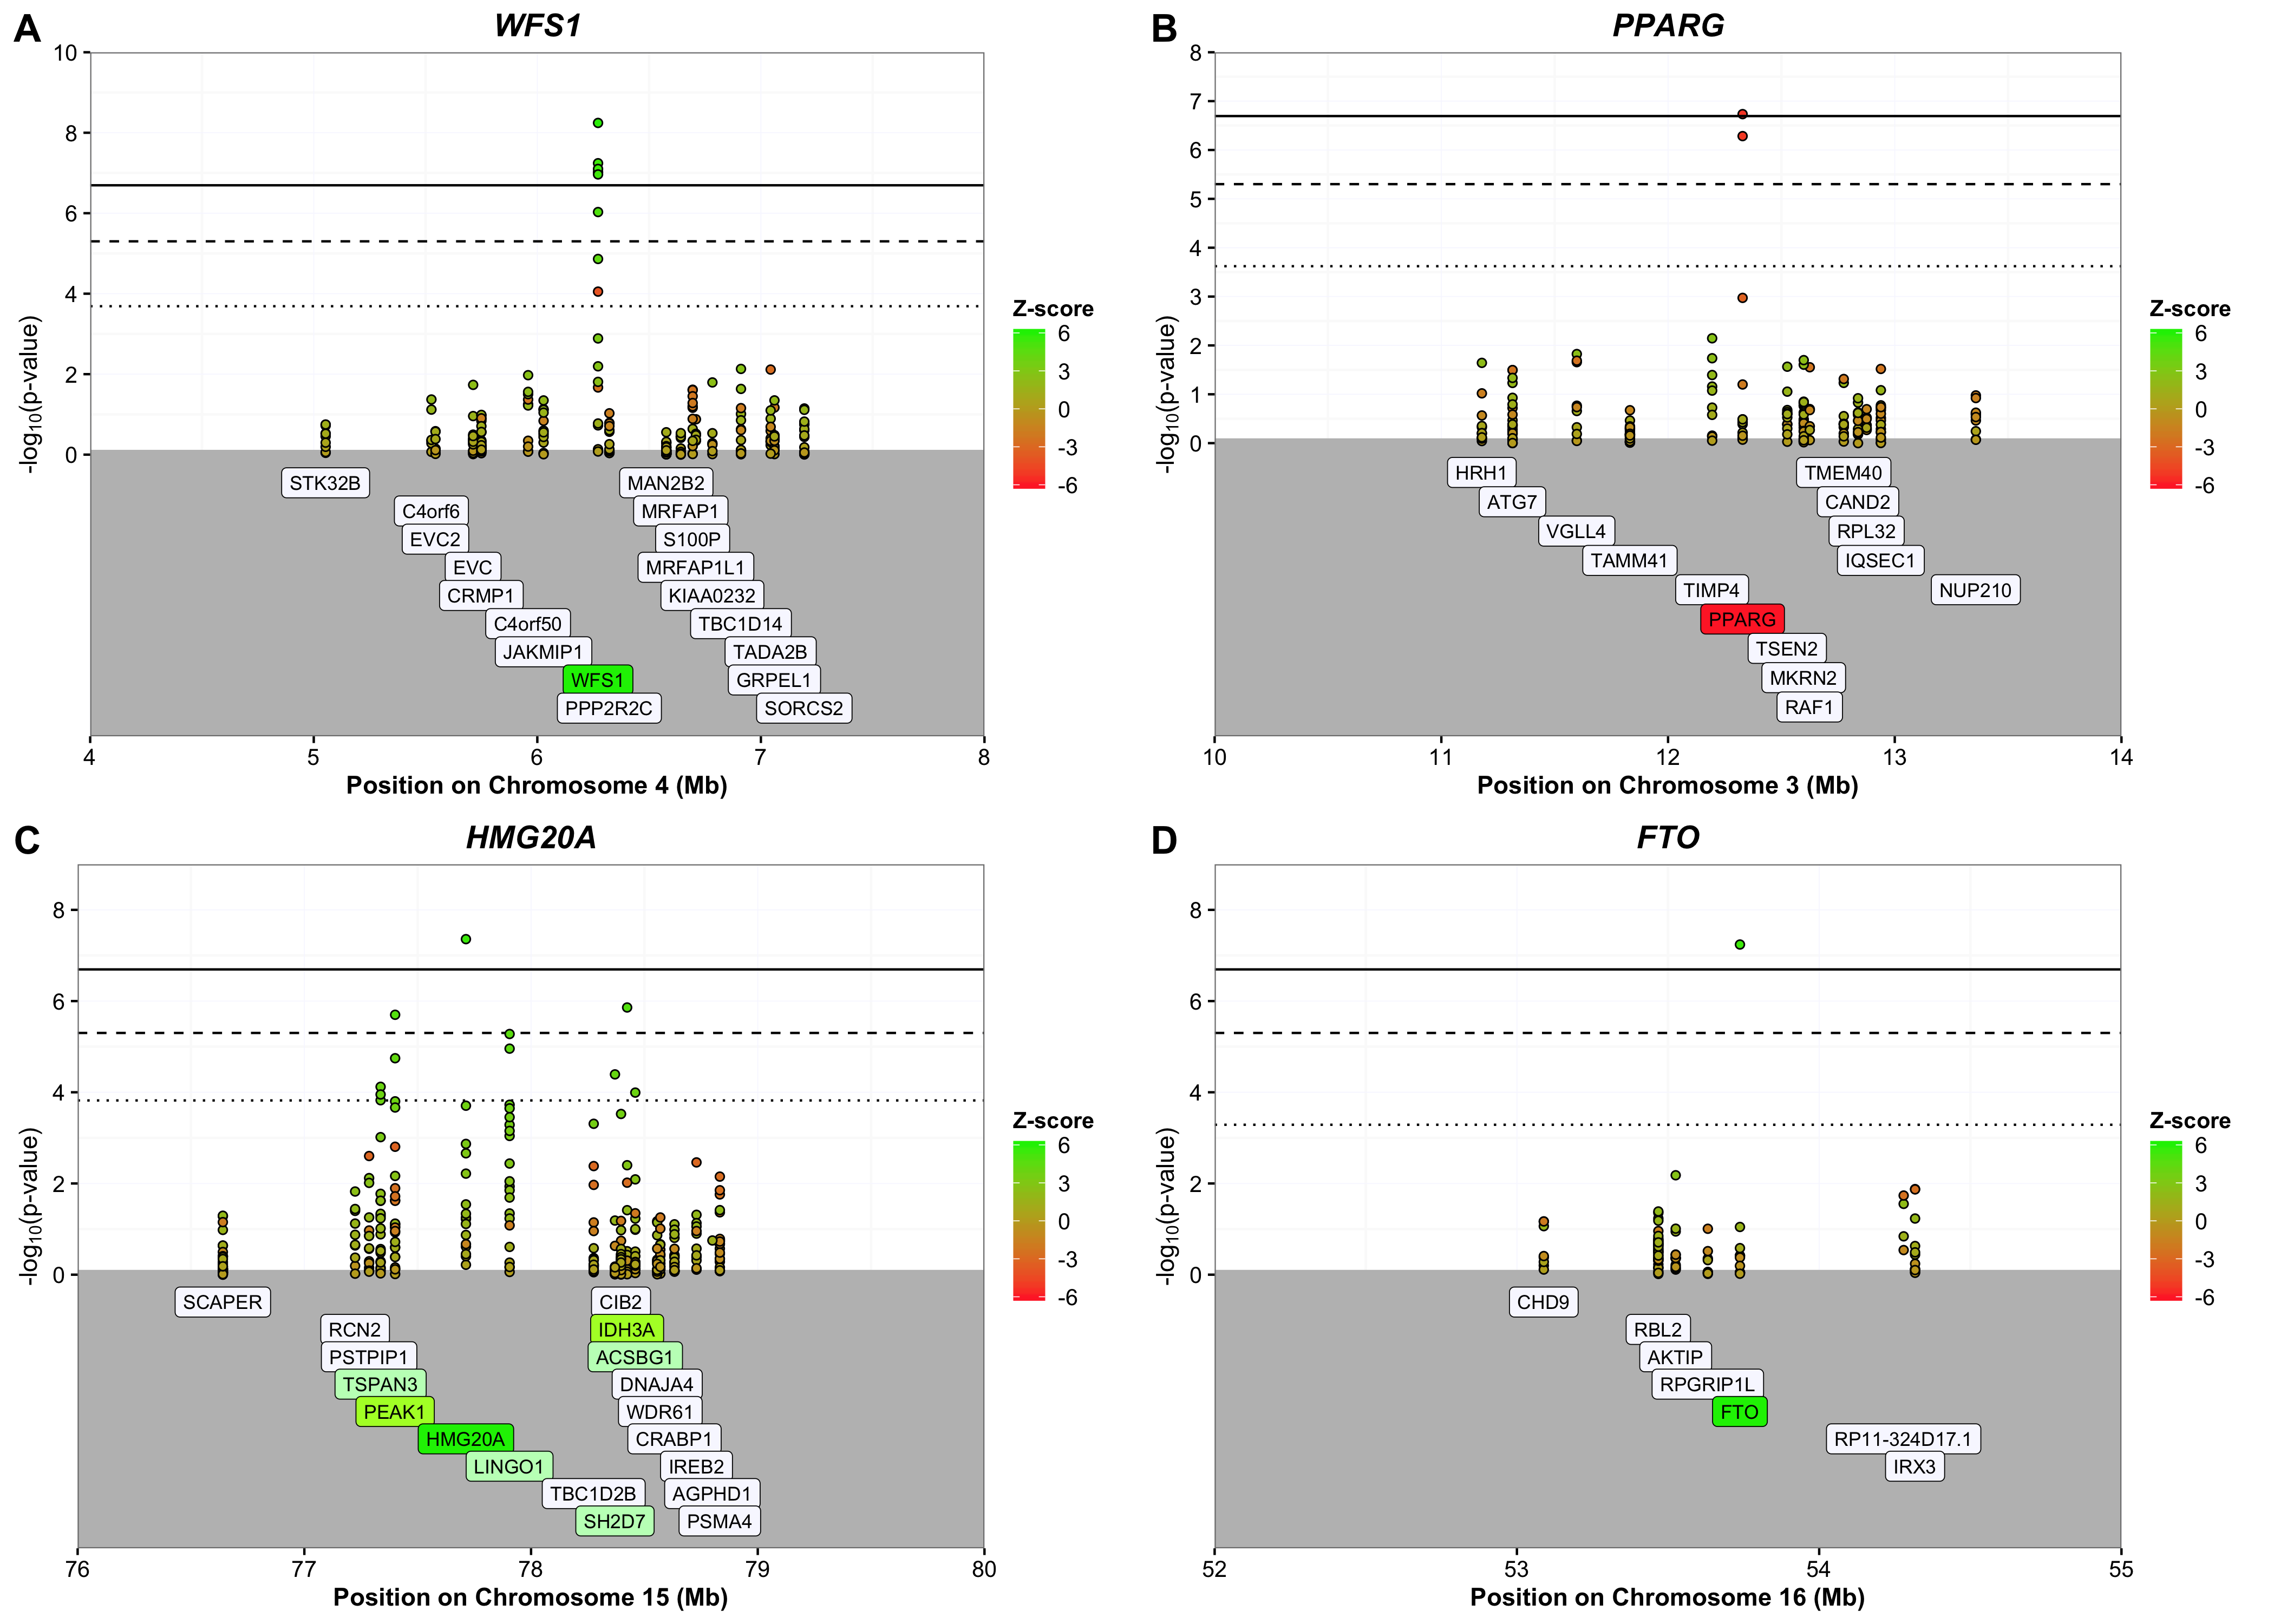
\includegraphics[width=\textwidth]{fig1_locusArray.png}
\caption{\textbf{Putative T2D genes supported by MetaXcan association in the DIAGRAM study.} We tested for association between predicted gene expression and T2D at $\sim2$ Mb genomic regions encompassing putative T2D genes implicated by the top $1,000$ SNPs associated with T2D from the DIAGRAM trans-ethnic meta-analysis of GWASs using $42$ tissue-level prediction models. Results are shown for regions where only the putative T2D gene is associated at the most stringent threshold: (A) \textit{WFS1}, (B) \textit{PPARG}, (C) \textit{HMG20A}, and (D) \textit{FTO}. The gene about which the genomic region is centered is indicated at the top of each panel. The solid, dashed, and dotted line denote significance correcting for the total number of tests performed across all models, genome-wide significance in a single model ($10,000$ tests), and locus-wide significance, respectively. Genomic position (Mb) and significance ($-\log_{10}$(p-value)) for each predicted gene expression value (from a particular tissue model) are shown on the $x$ and $y$-axis, respectively. Gene labels are shown in the gray region and are positioned at the transcription start site (TSS). Moreover, the color of each point corresponds to the magnitude and sign of the $Z$-score where positive and negative $Z$-scores are colored green and red, respectively. Similarly, gene labels are colored according to the Z-score of the most significant association at a gene if it meets locus-wide (light), genome-wide significance in at least one model (medium), or significance correcting for the total number of tests performed across all models (dark). } 
\label{fig:locus_array_1}
\end{figure}


%Figure 2 
\begin{figure}
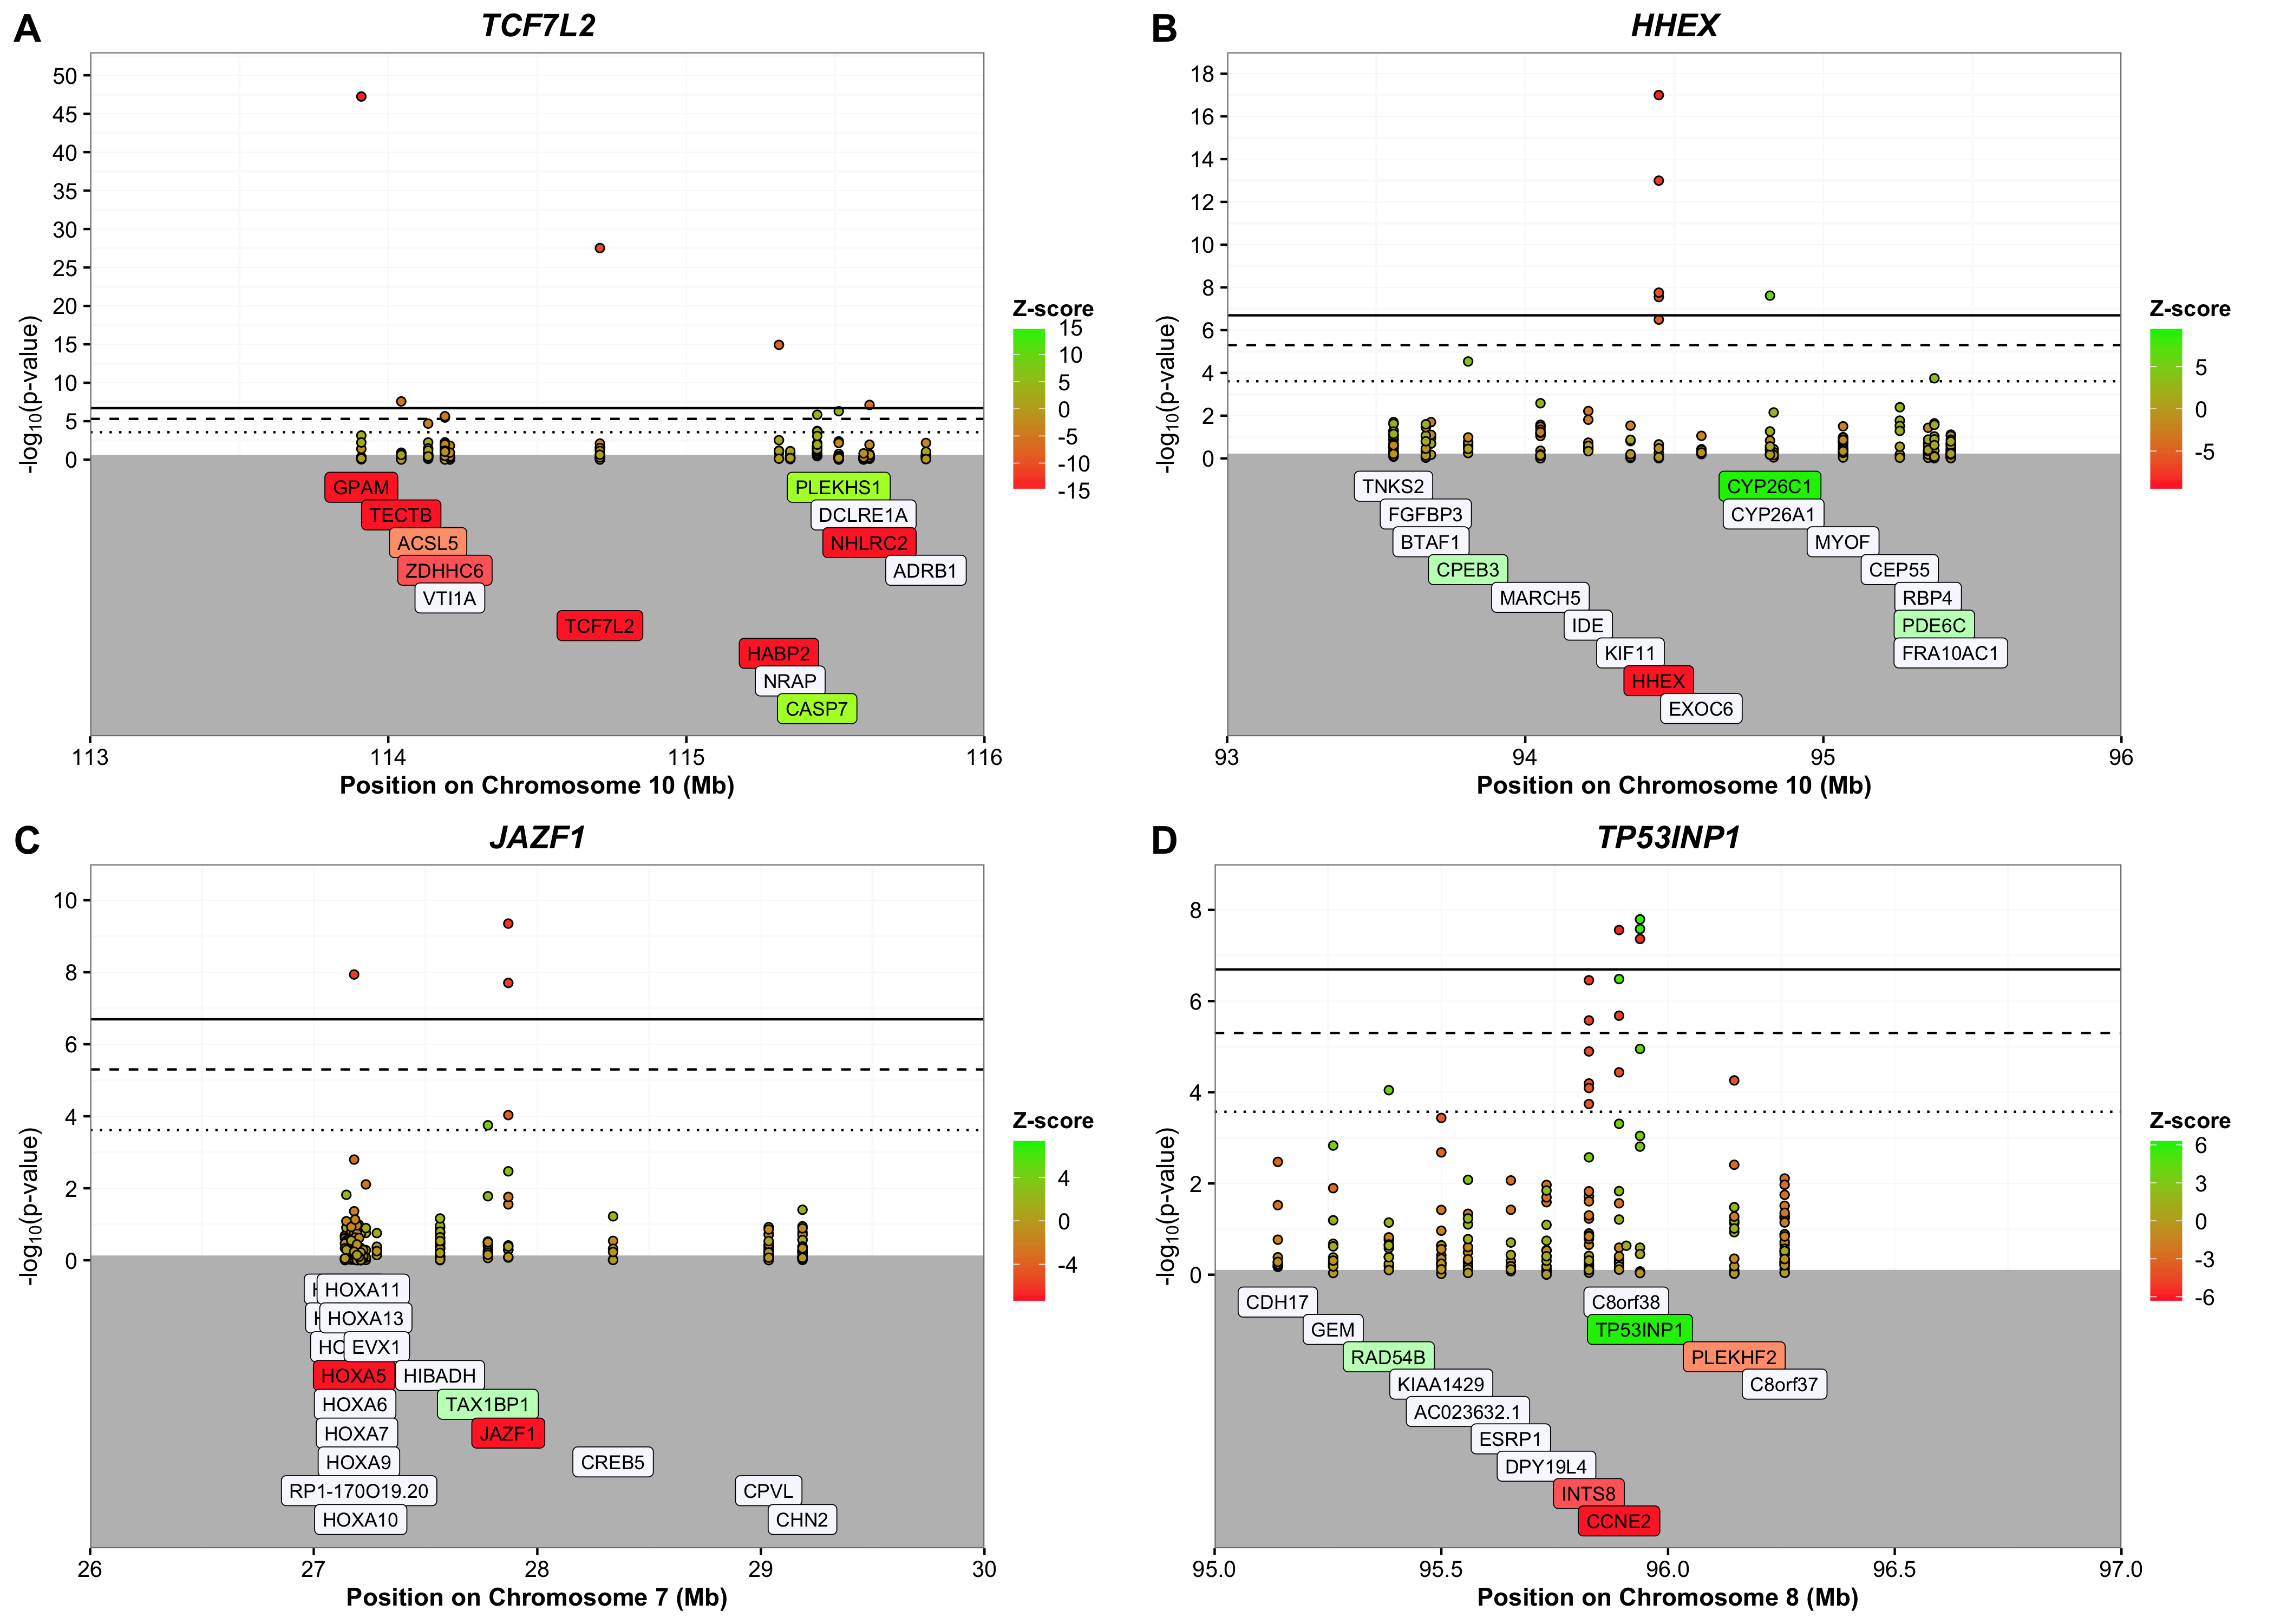
\includegraphics[width=\textwidth]{fig2_locusArray.png}
\caption{\textbf{Regions harboring MetaXcan associations with putative T2D genes and novel candidate T2D genes.} We tested for association between predicted gene expression and T2D at $\sim2$ Mb genomic regions encompassing putative T2D genes implicated by the top $1,000$ SNPs associated with T2D from the DIAGRAM trans-ethnic meta-analysis of GWASs using $42$ tissue-level prediction models. Results are shown for regions where both the putative T2D gene and unreported T2D genes are associated at the most stringent threshold: (A) \textit{TCF7L2}, (B) \textit{HHEX}, (C) \textit{JAZF1}, and (D) \textit{TP53INP1}. The gene about which the genomic region is centered is indicated at the top of each panel. The solid, dashed, and dotted line denote significance correcting for the total number of tests performed across all models, genome-wide significance in a single model ($10,000$ tests), and locus-wide significance, respectively. Genomic position (Mb) and significance ($-\log_{10}$(p-value)) for each predicted gene expression value (from a particular tissue model) are shown on the $x$ and $y$-axis, respectively. Gene labels are shown in the gray region and are positioned at the transcription start site (TSS). Moreover, the color of each point corresponds to the magnitude and sign of the $Z$-score where positive and negative $Z$-scores are colored green and red, respectively. Similarly, gene labels are colored according to the Z-score of the most significant association at a gene if it meets locus-wide (light), genome-wide significance in at least one model (medium), or significance correcting for the total number of tests performed across all models (dark). } 
\label{fig:locus_array_2}
\end{figure}
% Figure 3 
\begin{figure}
	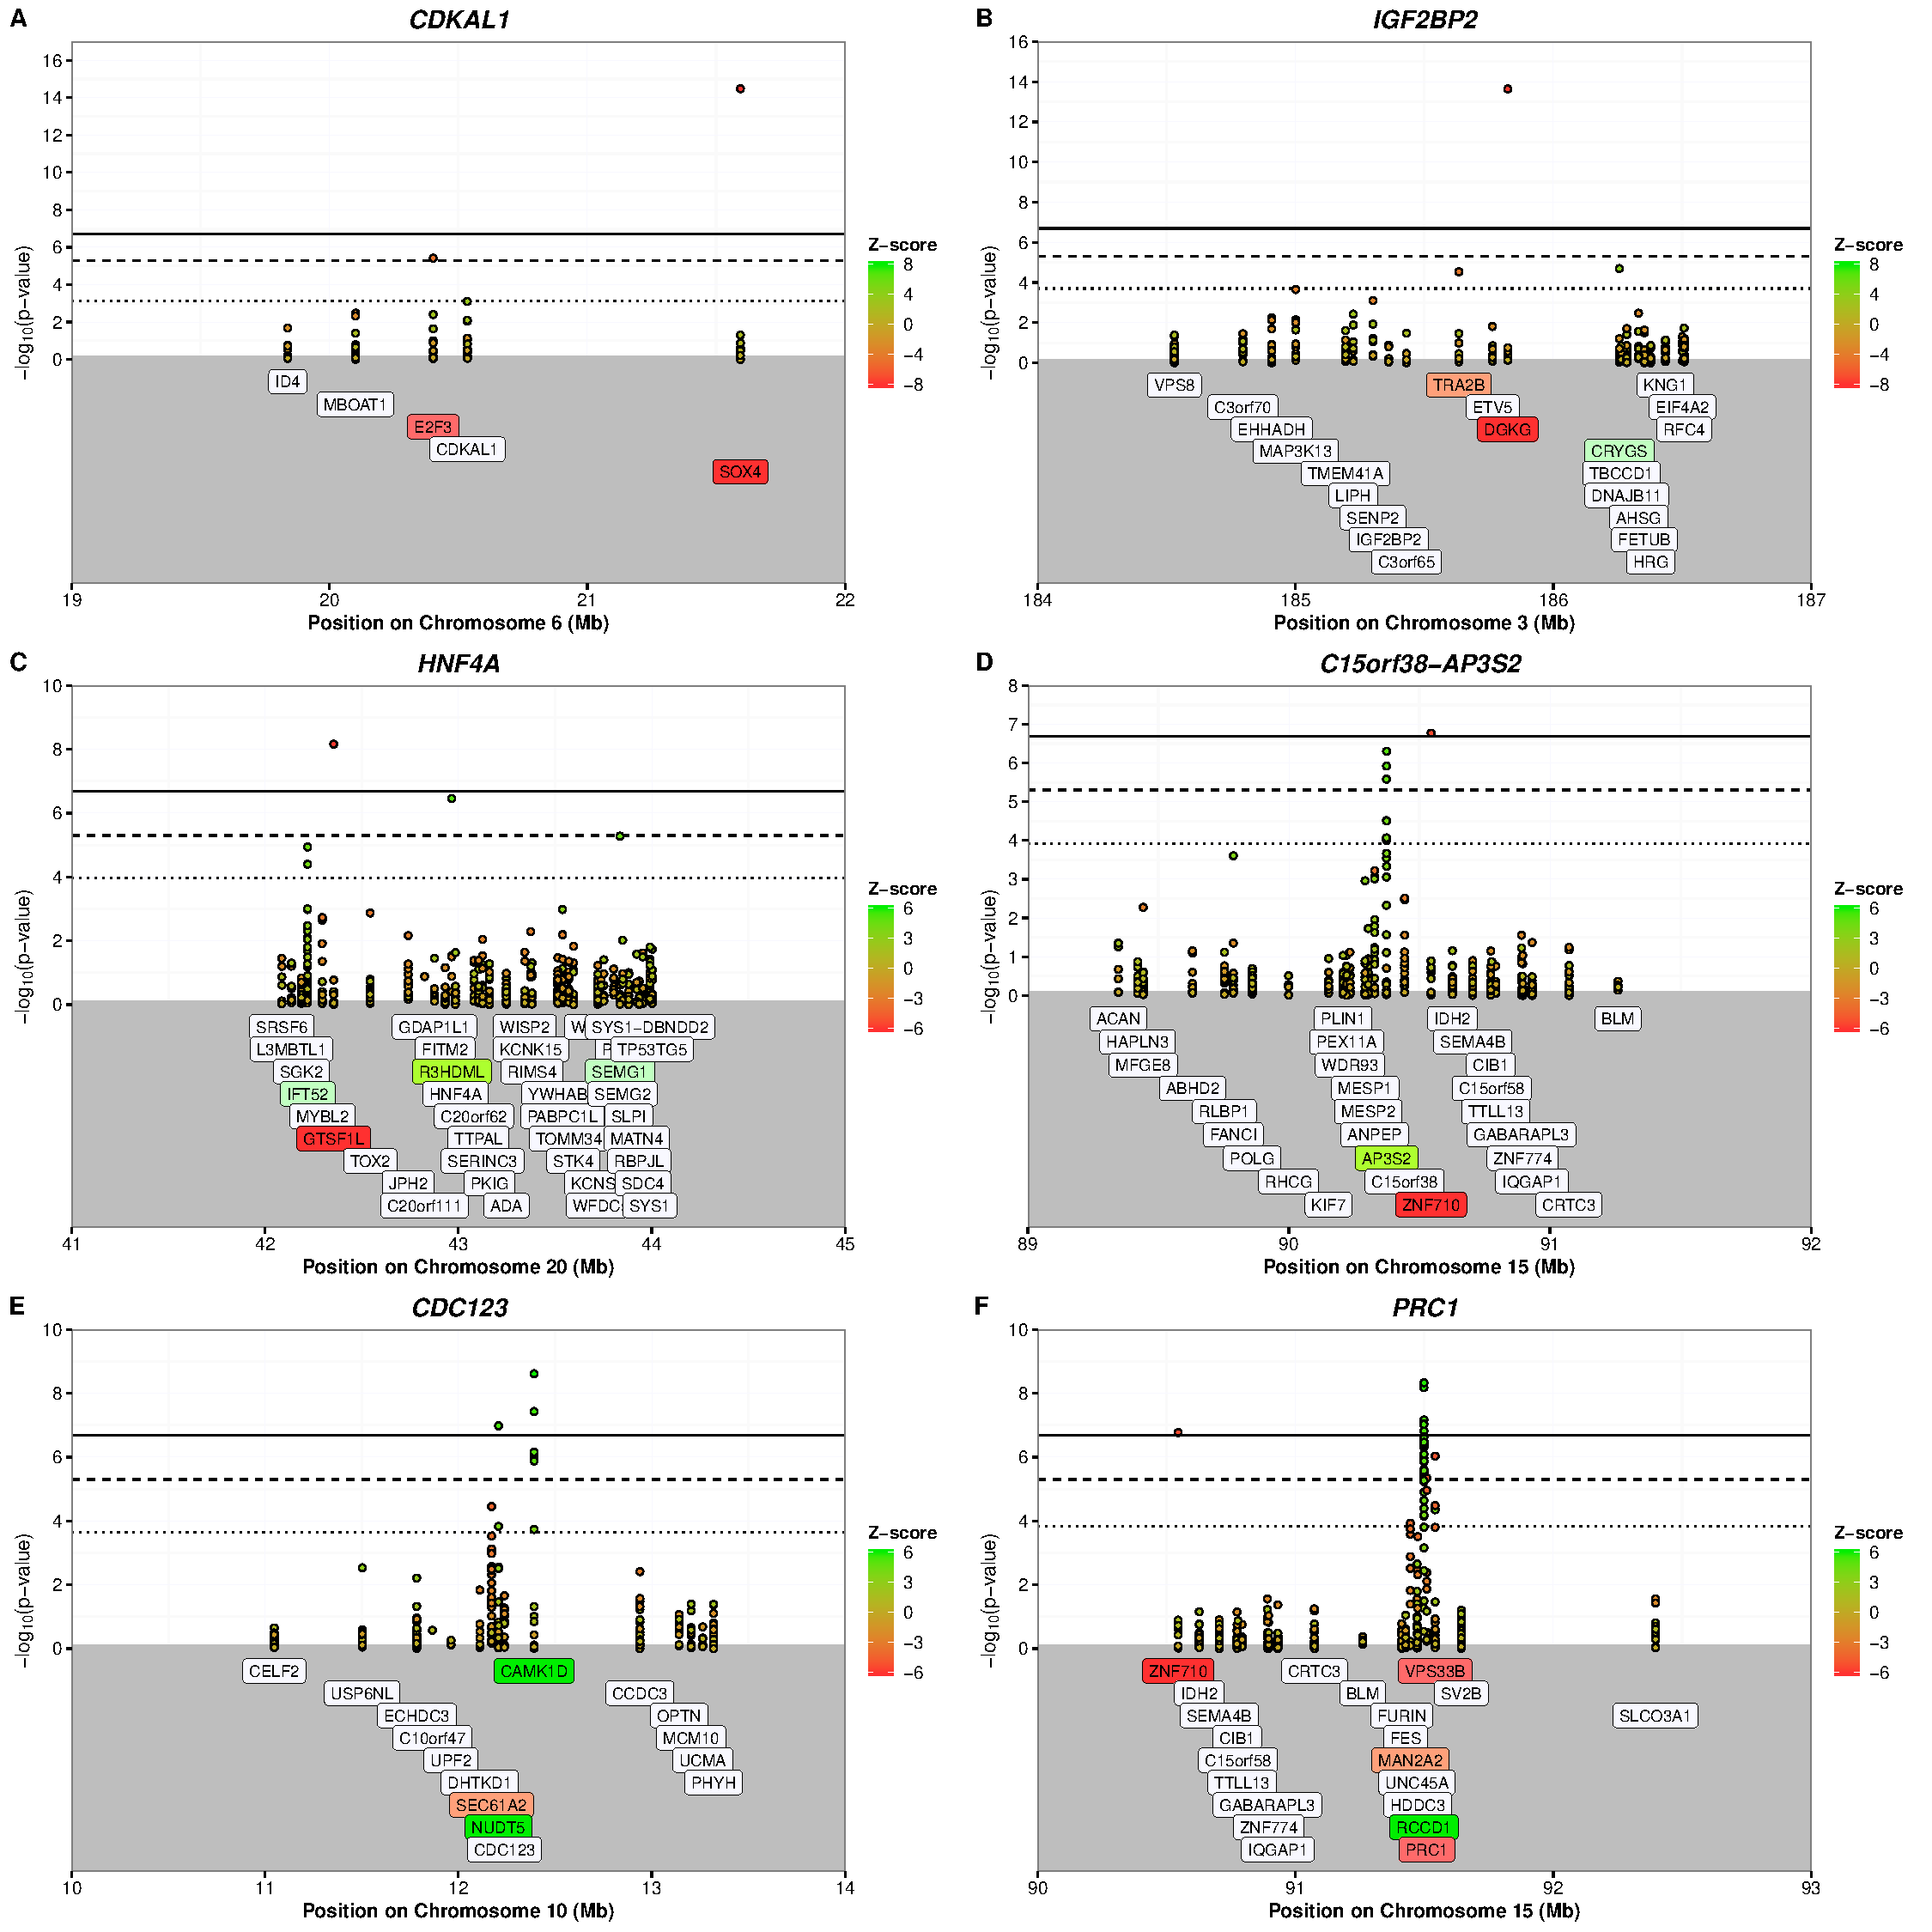
\includegraphics[width=\textwidth]{fig3_locusArray.pdf}
	\caption{\textbf{Regions where non-putative T2D genes show strong MetaXcan association with T2D.} Results are shown for regions where unreported T2D genes are associated at the most stringent threshold: (A) \textit{CDKAL1}, (B) \textit{IGF2BP2}, (C) \textit{HNF4A}, (D) \textit{C15orf38-AP3S2}, (E) \textit{CDC123}, and (F) \textit{PRC1}. The solid, dashed, and dotted line denote significance correcting for the total number of tests performed across all models, genome-wide significance in a single model ($10,000$ tests), and locus-wide significance, respectively. Genomic position (Mb) and significance ($-\log_{10}$(p-value)) for each predicted gene expression value (from a particular tissue model) are shown on the $x$ and $y$-axis, respectively. Gene labels are shown in the gray region and are positioned at the transcription start site (TSS). Moreover, the color of each point corresponds to the magnitude and sign of the $Z$-score where positive and negative $Z$-scores are colored green and red, respectively}
    \label{fig:locus_array_3}
\end{figure}

% Figure 3 
\begin{figure}
	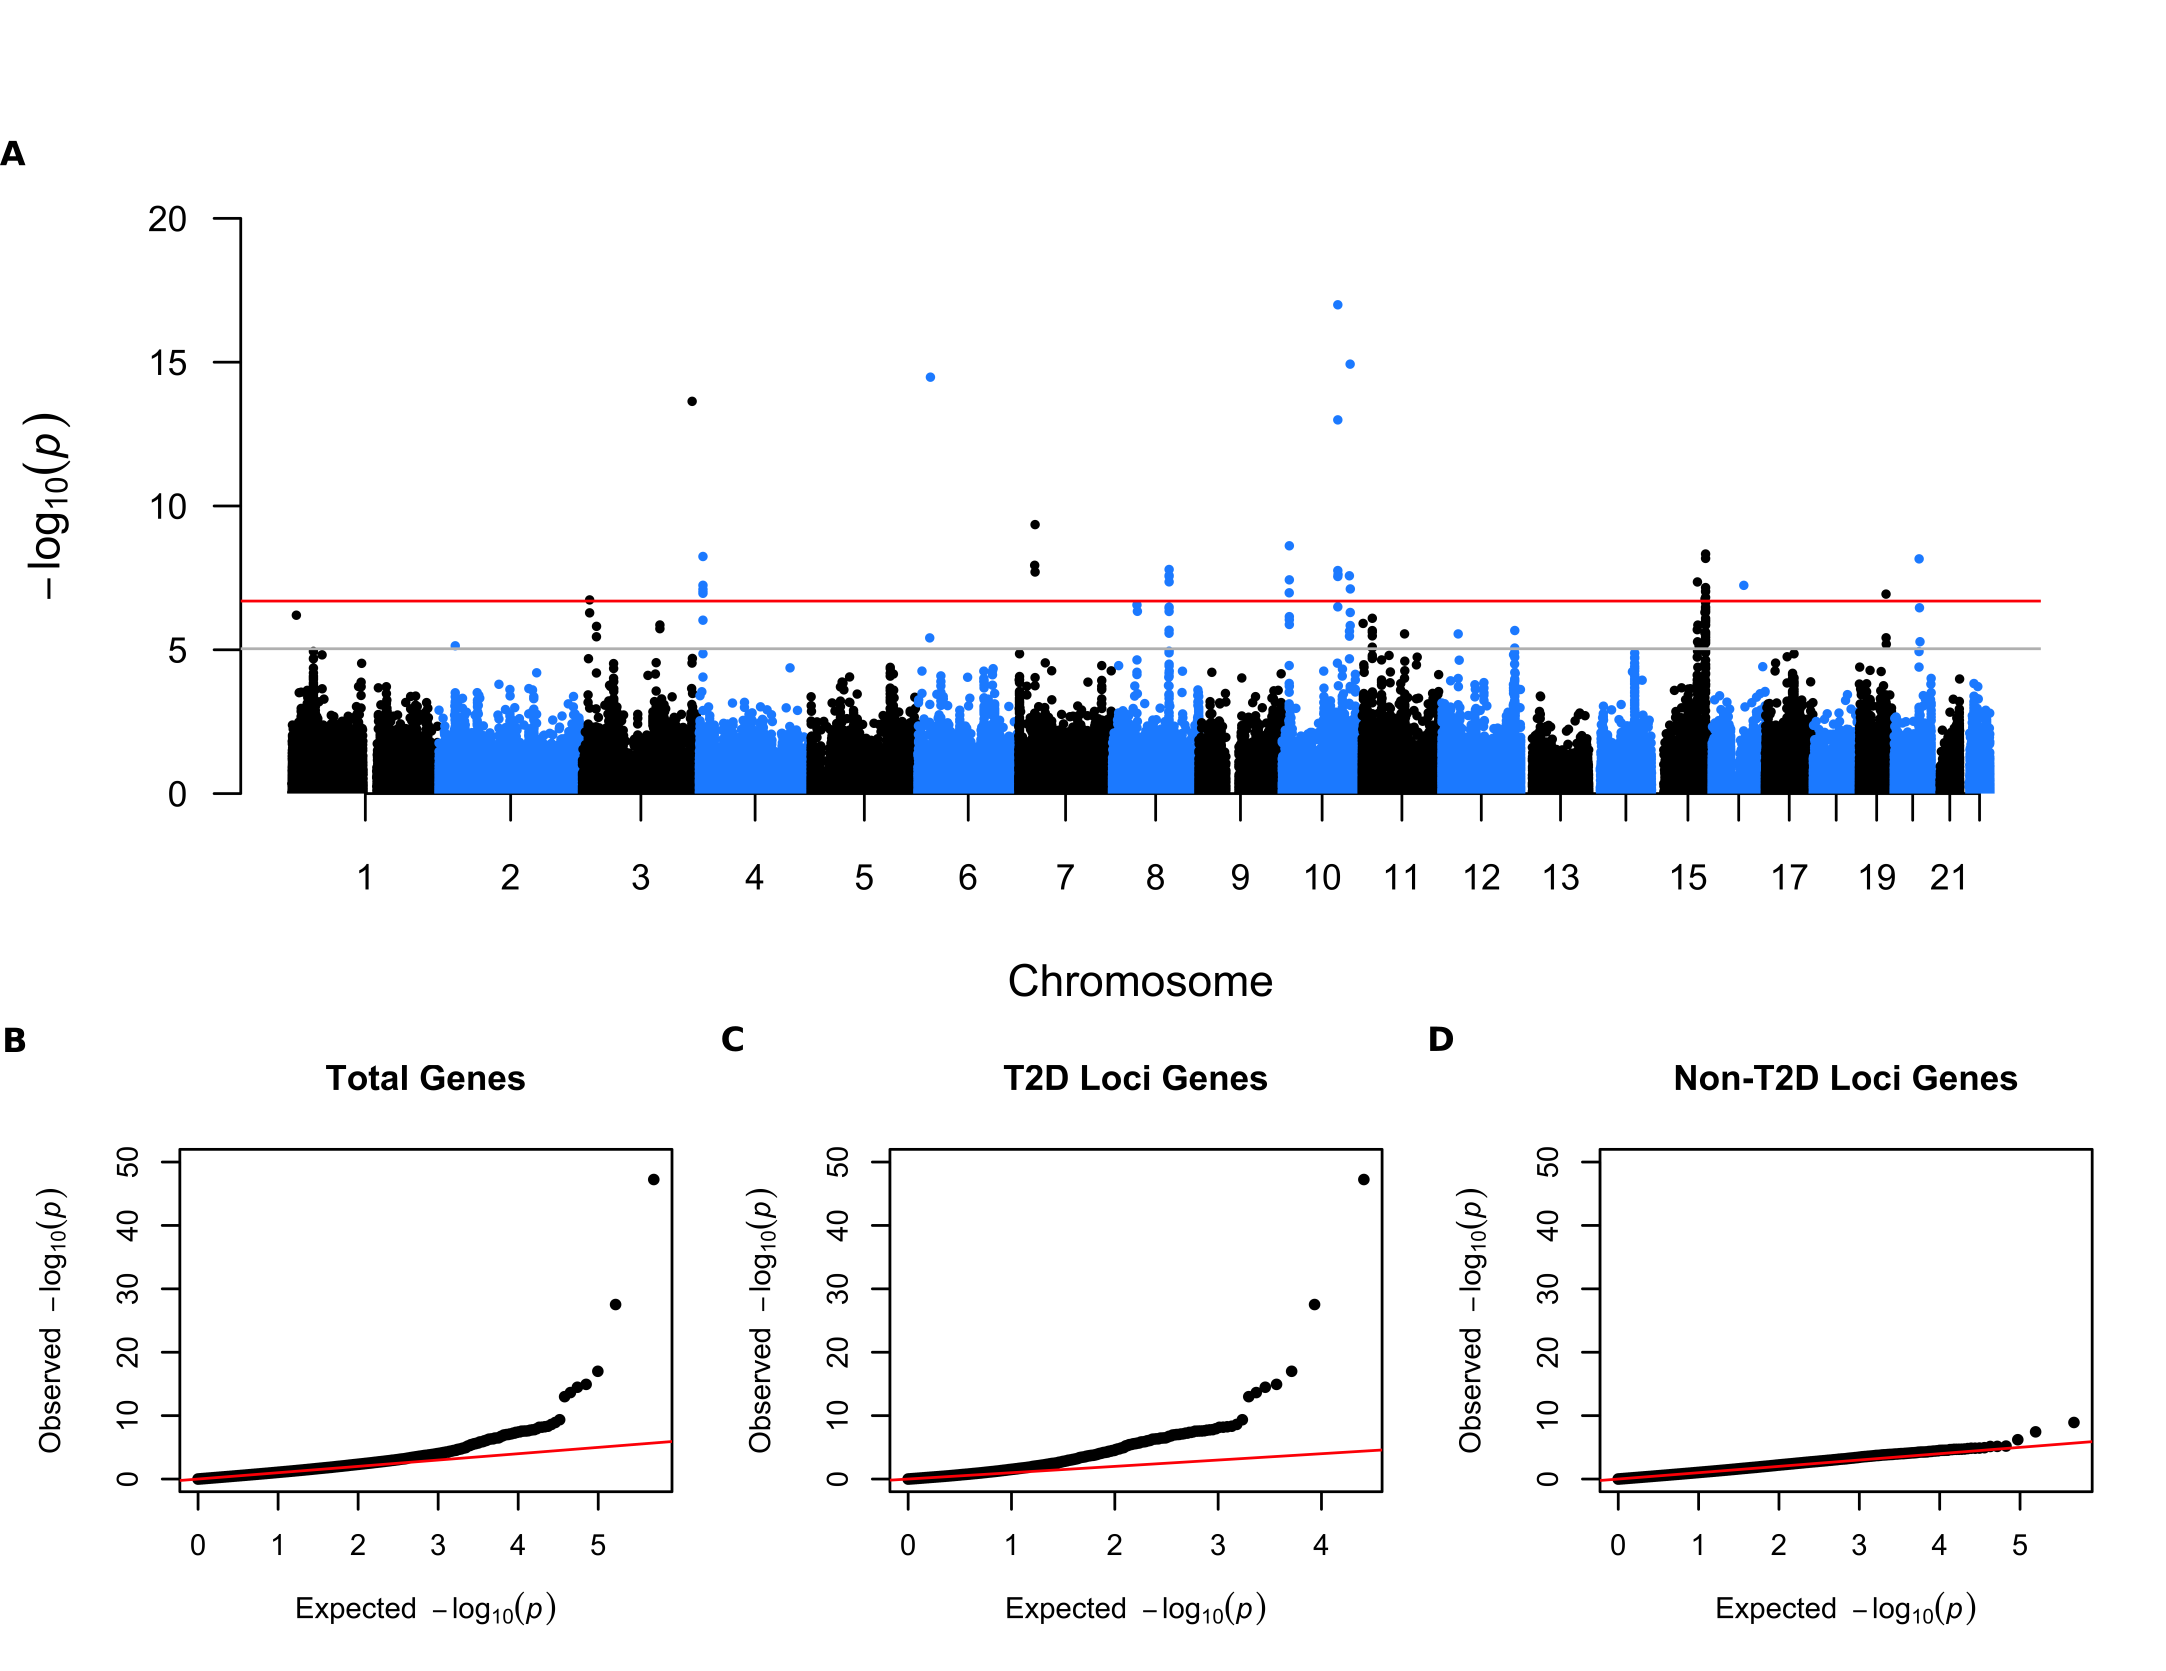
\includegraphics[width=\textwidth]{fig4_manhat_qqArray.png}
	\caption{\textbf{Genome-wide MetaXcan analyses shows gene associations constrained to putative T2D loci.} We used MetaXcan to estimate gene expression and test for T2D association in the DIAGRAM trans-ethnic meta-analysis summary dataset for each of $42$ predictive models (i.e. $42$ separate association tests). (A) Manhattan plot showing significance ($-\log_{10}$(p-value)) of associations between predicted expression and T2D. Results across all tissue-level analyses are shown. The solid red line denotes significance threshold corrected for the total number of individual tests performed across all models and the solid gray line denotes the suggestive line corresponding to significance in at least one model (i.e. $10,000$ tests). (B) QQ-plot showing the expected versus observed distribution of $-\log_{10}$(p-value) for each predicted gene expression trait across all $42$ association tests. (C) QQ-plot showing the expected versus observed distribution of $-\log_{10}$(p-value) across all $42$ association tests for all genes within 1 Mb of T2D-associated SNPs. (D) QQ-plot showing the expected versus observed distribution of $-\log_{10}$(p-value) across all $42$ association tests for all genes exceeding $1$ Mb of T2D-associated SNPs.}
    \label{fig:manhat_qqarray}
\end{figure}

% Table 1 
\begin{table}
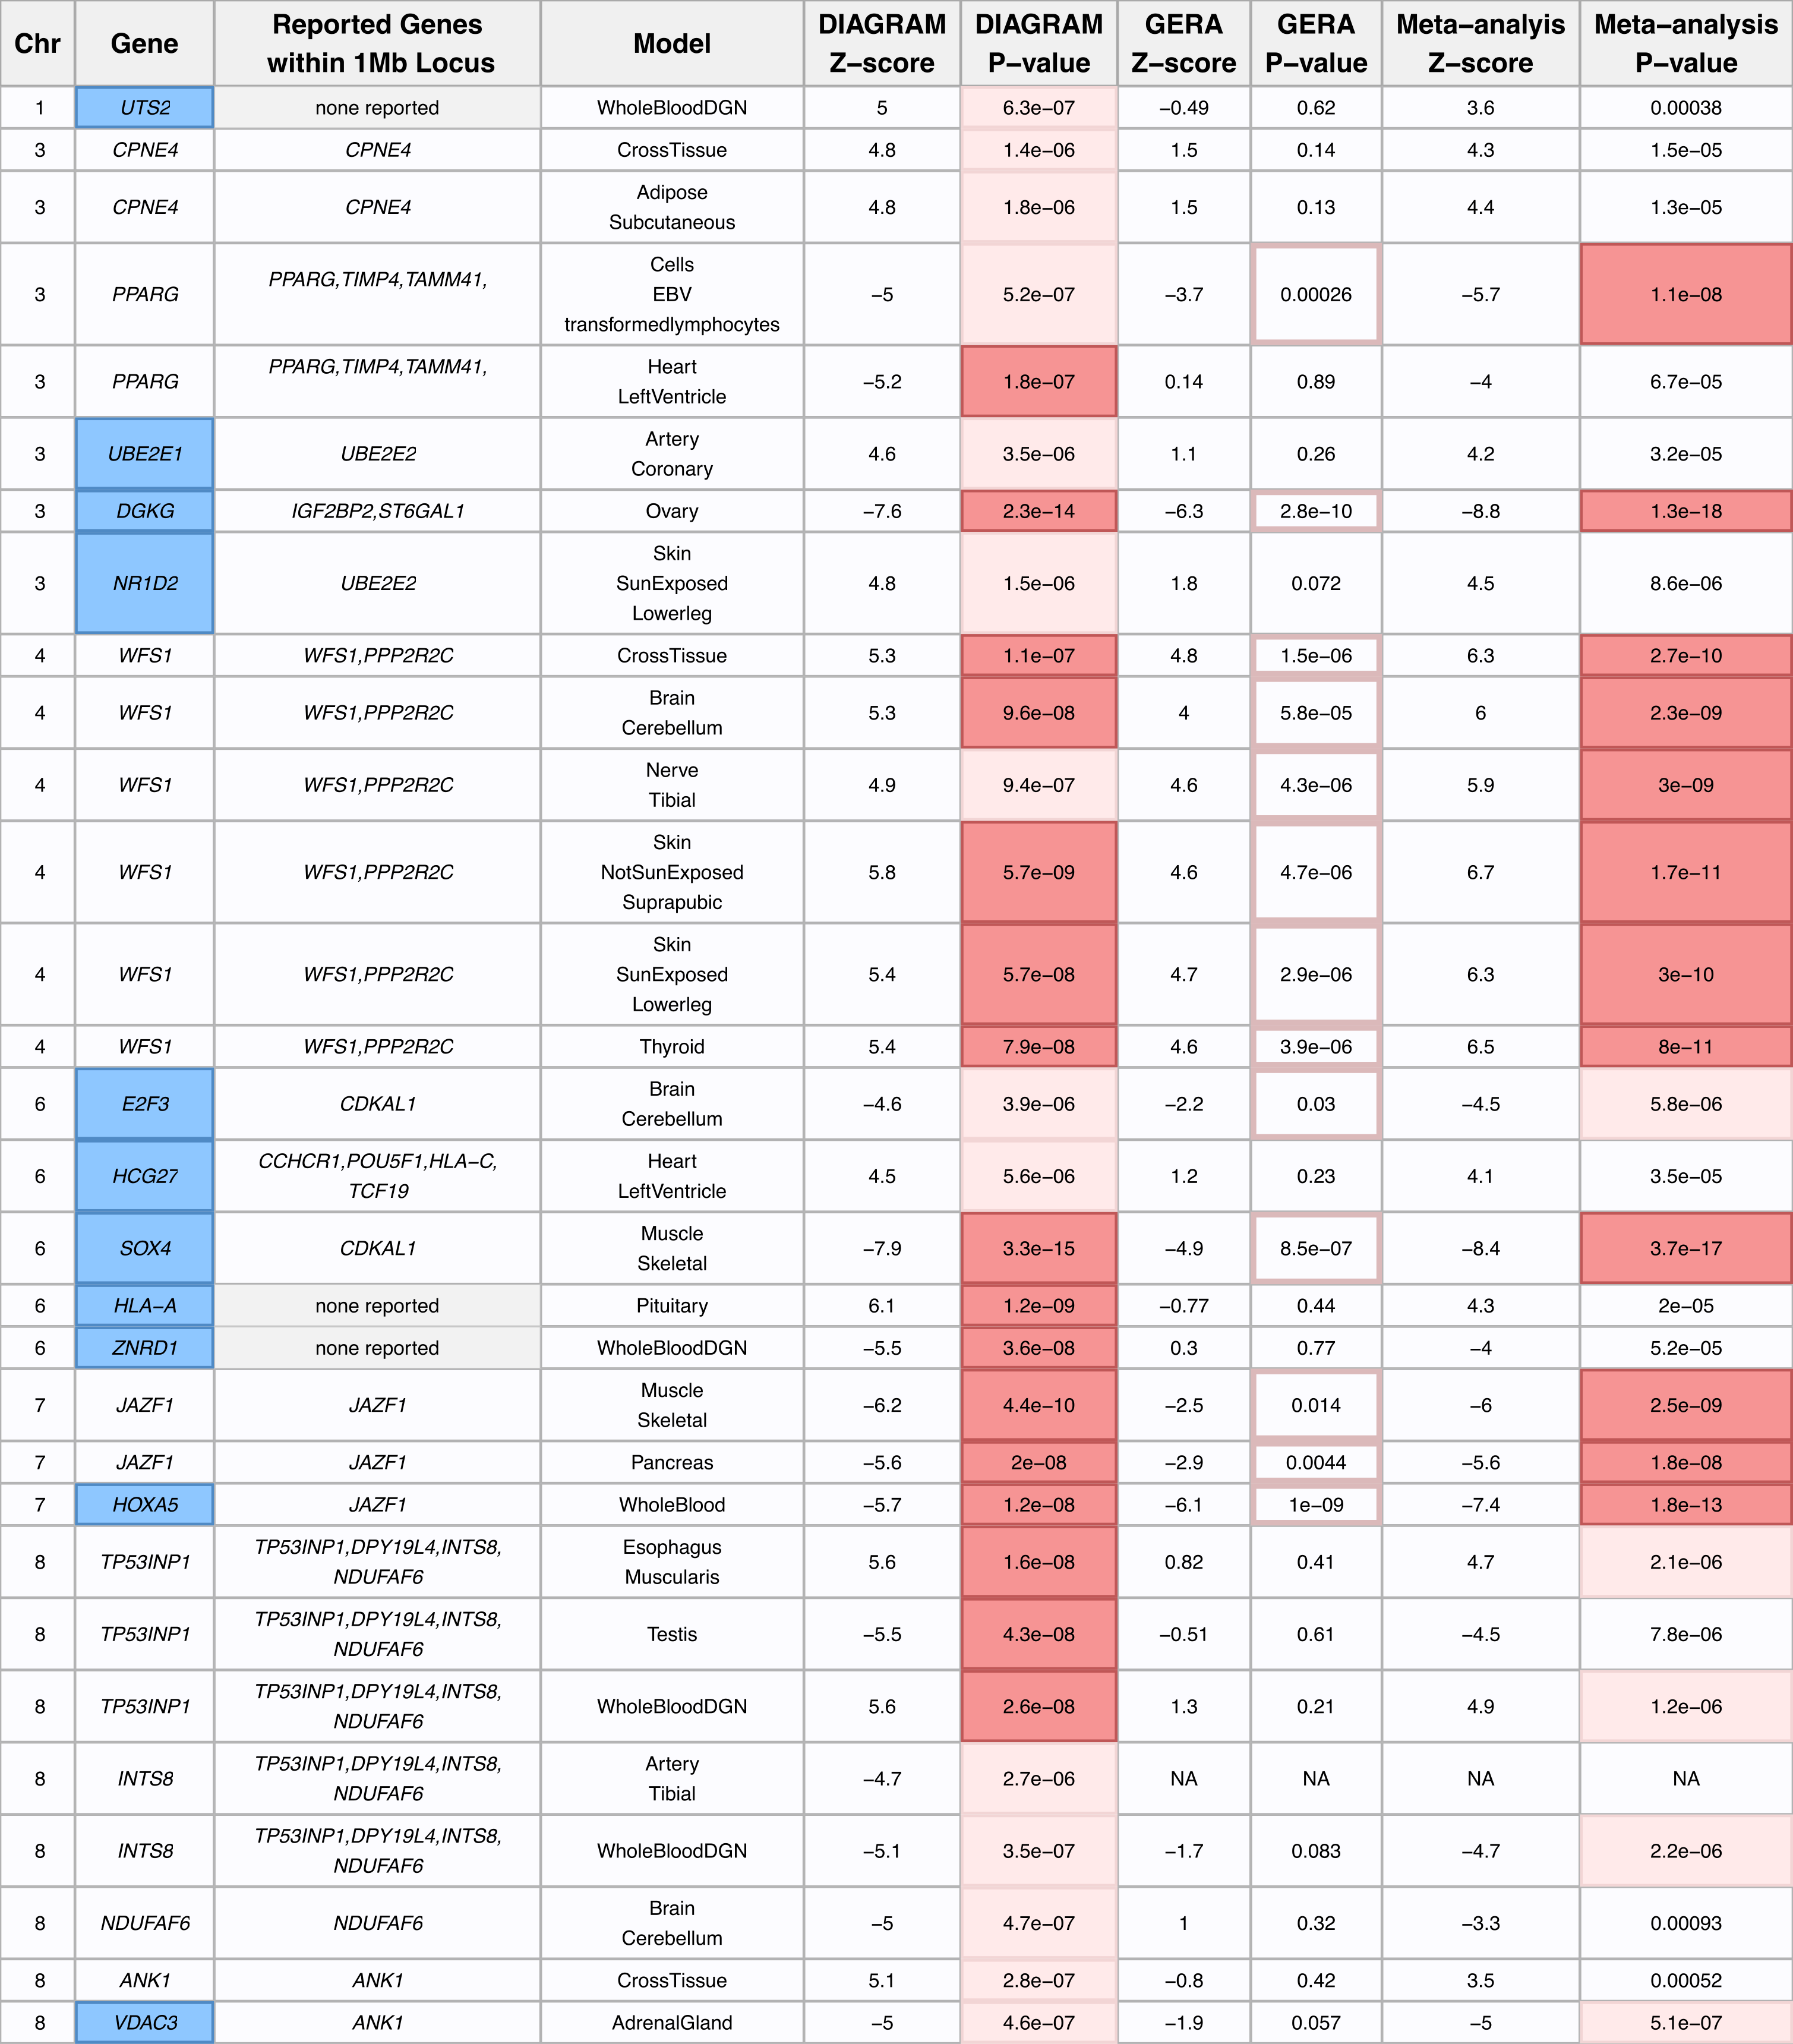
\includegraphics[width=0.95\textwidth]{table1_part1.png}
\caption{\textbf{MetaXcan associations with T2D.} Results for genes and corresponding models that meet genome-wide significance \textit{in at least one model} from the DIAGRAM analysis are shown with nearby genes and results from the GERA replication study and meta-analysis of DIAGRAM and GERA Metaxcan associations. Blue shading denotes genes not implicated by the top $1,000$ SNPs from the DIAGRAM trans-ethnic meta-analysis of GWASs. Pink and red shading denote genome-wide significance in one model and across all models, respectively, for the DIAGRAM and meta-analysis. Replication in the GERA study is denoted by a pink outline.} 
\label{tab:table1.part1}
\end{table}

\begin{table}
\ContinuedFloat
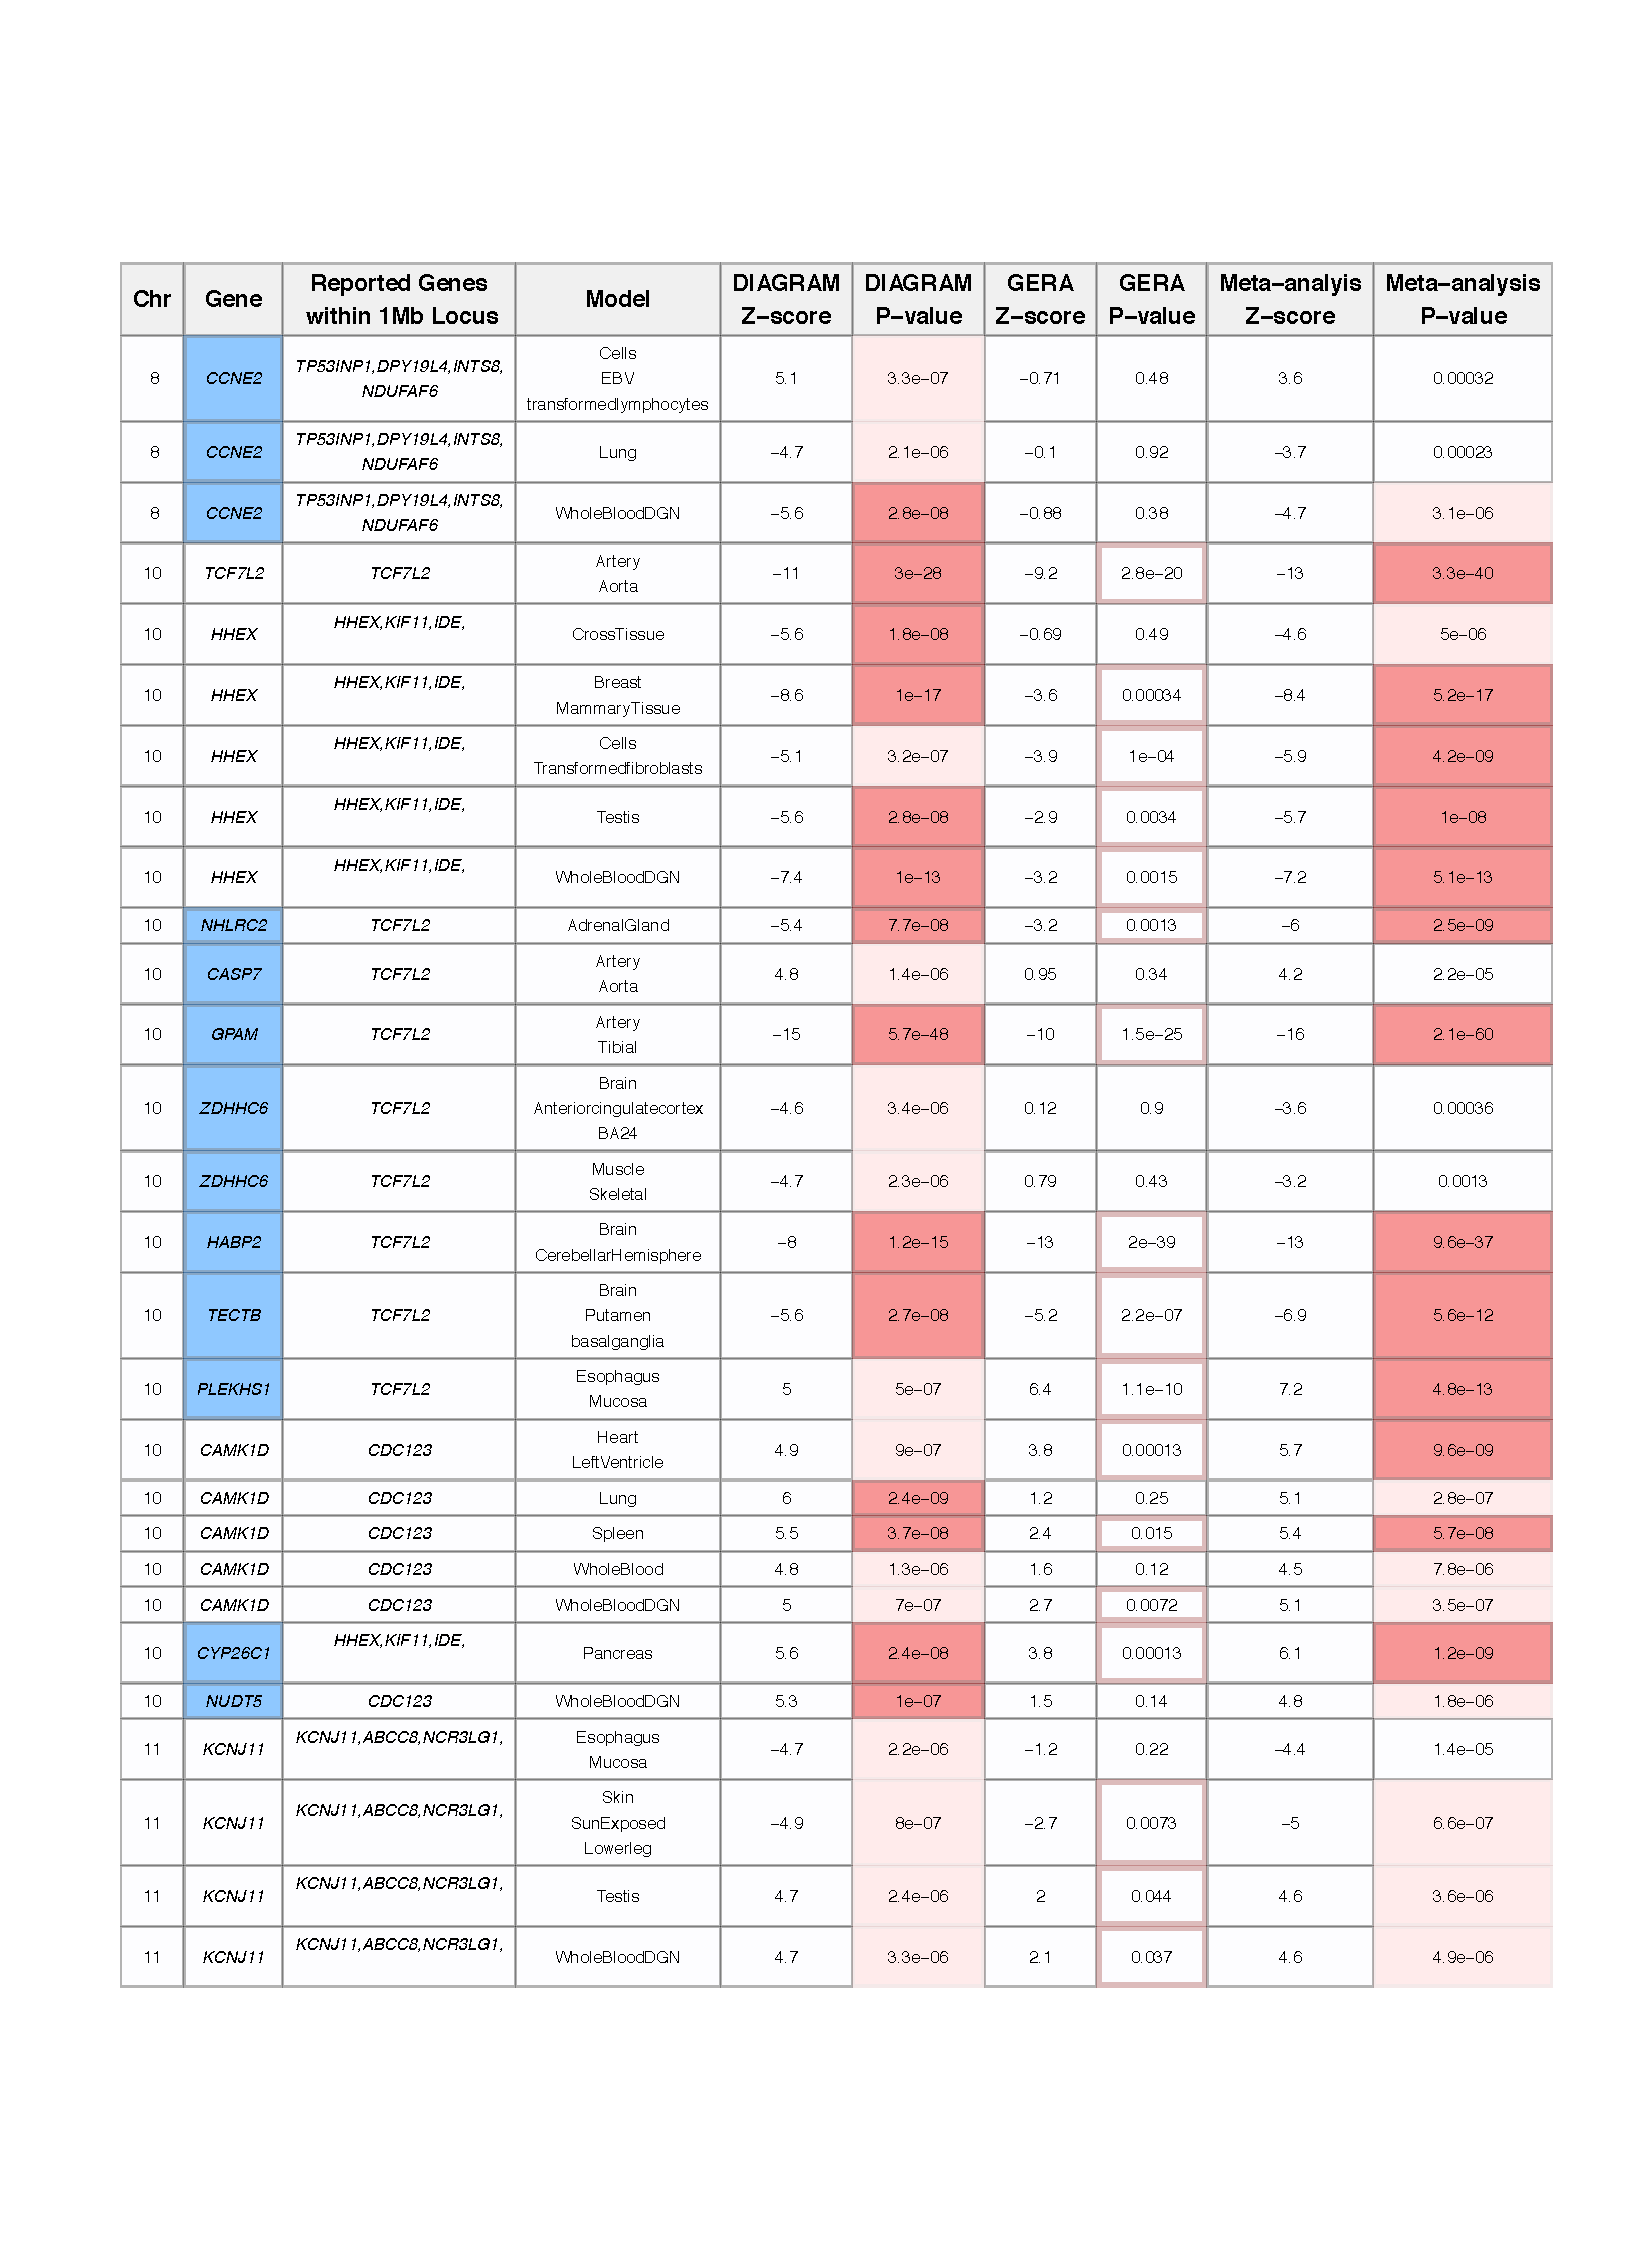
\includegraphics[width=0.91\textwidth]{table1_part2.pdf}
\caption{\textbf{MetaXcan associations with T2D.} Results for genes and corresponding models that meet genome-wide significance \textit{in at least one model} from the DIAGRAM analysis are shown with nearby genes and results from the GERA replication study and meta-analysis of DIAGRAM and GERA Metaxcan associations. Blue shading denotes genes not implicated by the top $1,000$ SNPs from the DIAGRAM trans-ethnic meta-analysis of GWASs. Pink and red shading denote genome-wide significance in one model and across all models, respectively, for the DIAGRAM and meta-analysis. Replication in the GERA study is denoted by a pink outline.} \label{tab:table1.part2}
\end{table}

\begin{table}
\ContinuedFloat
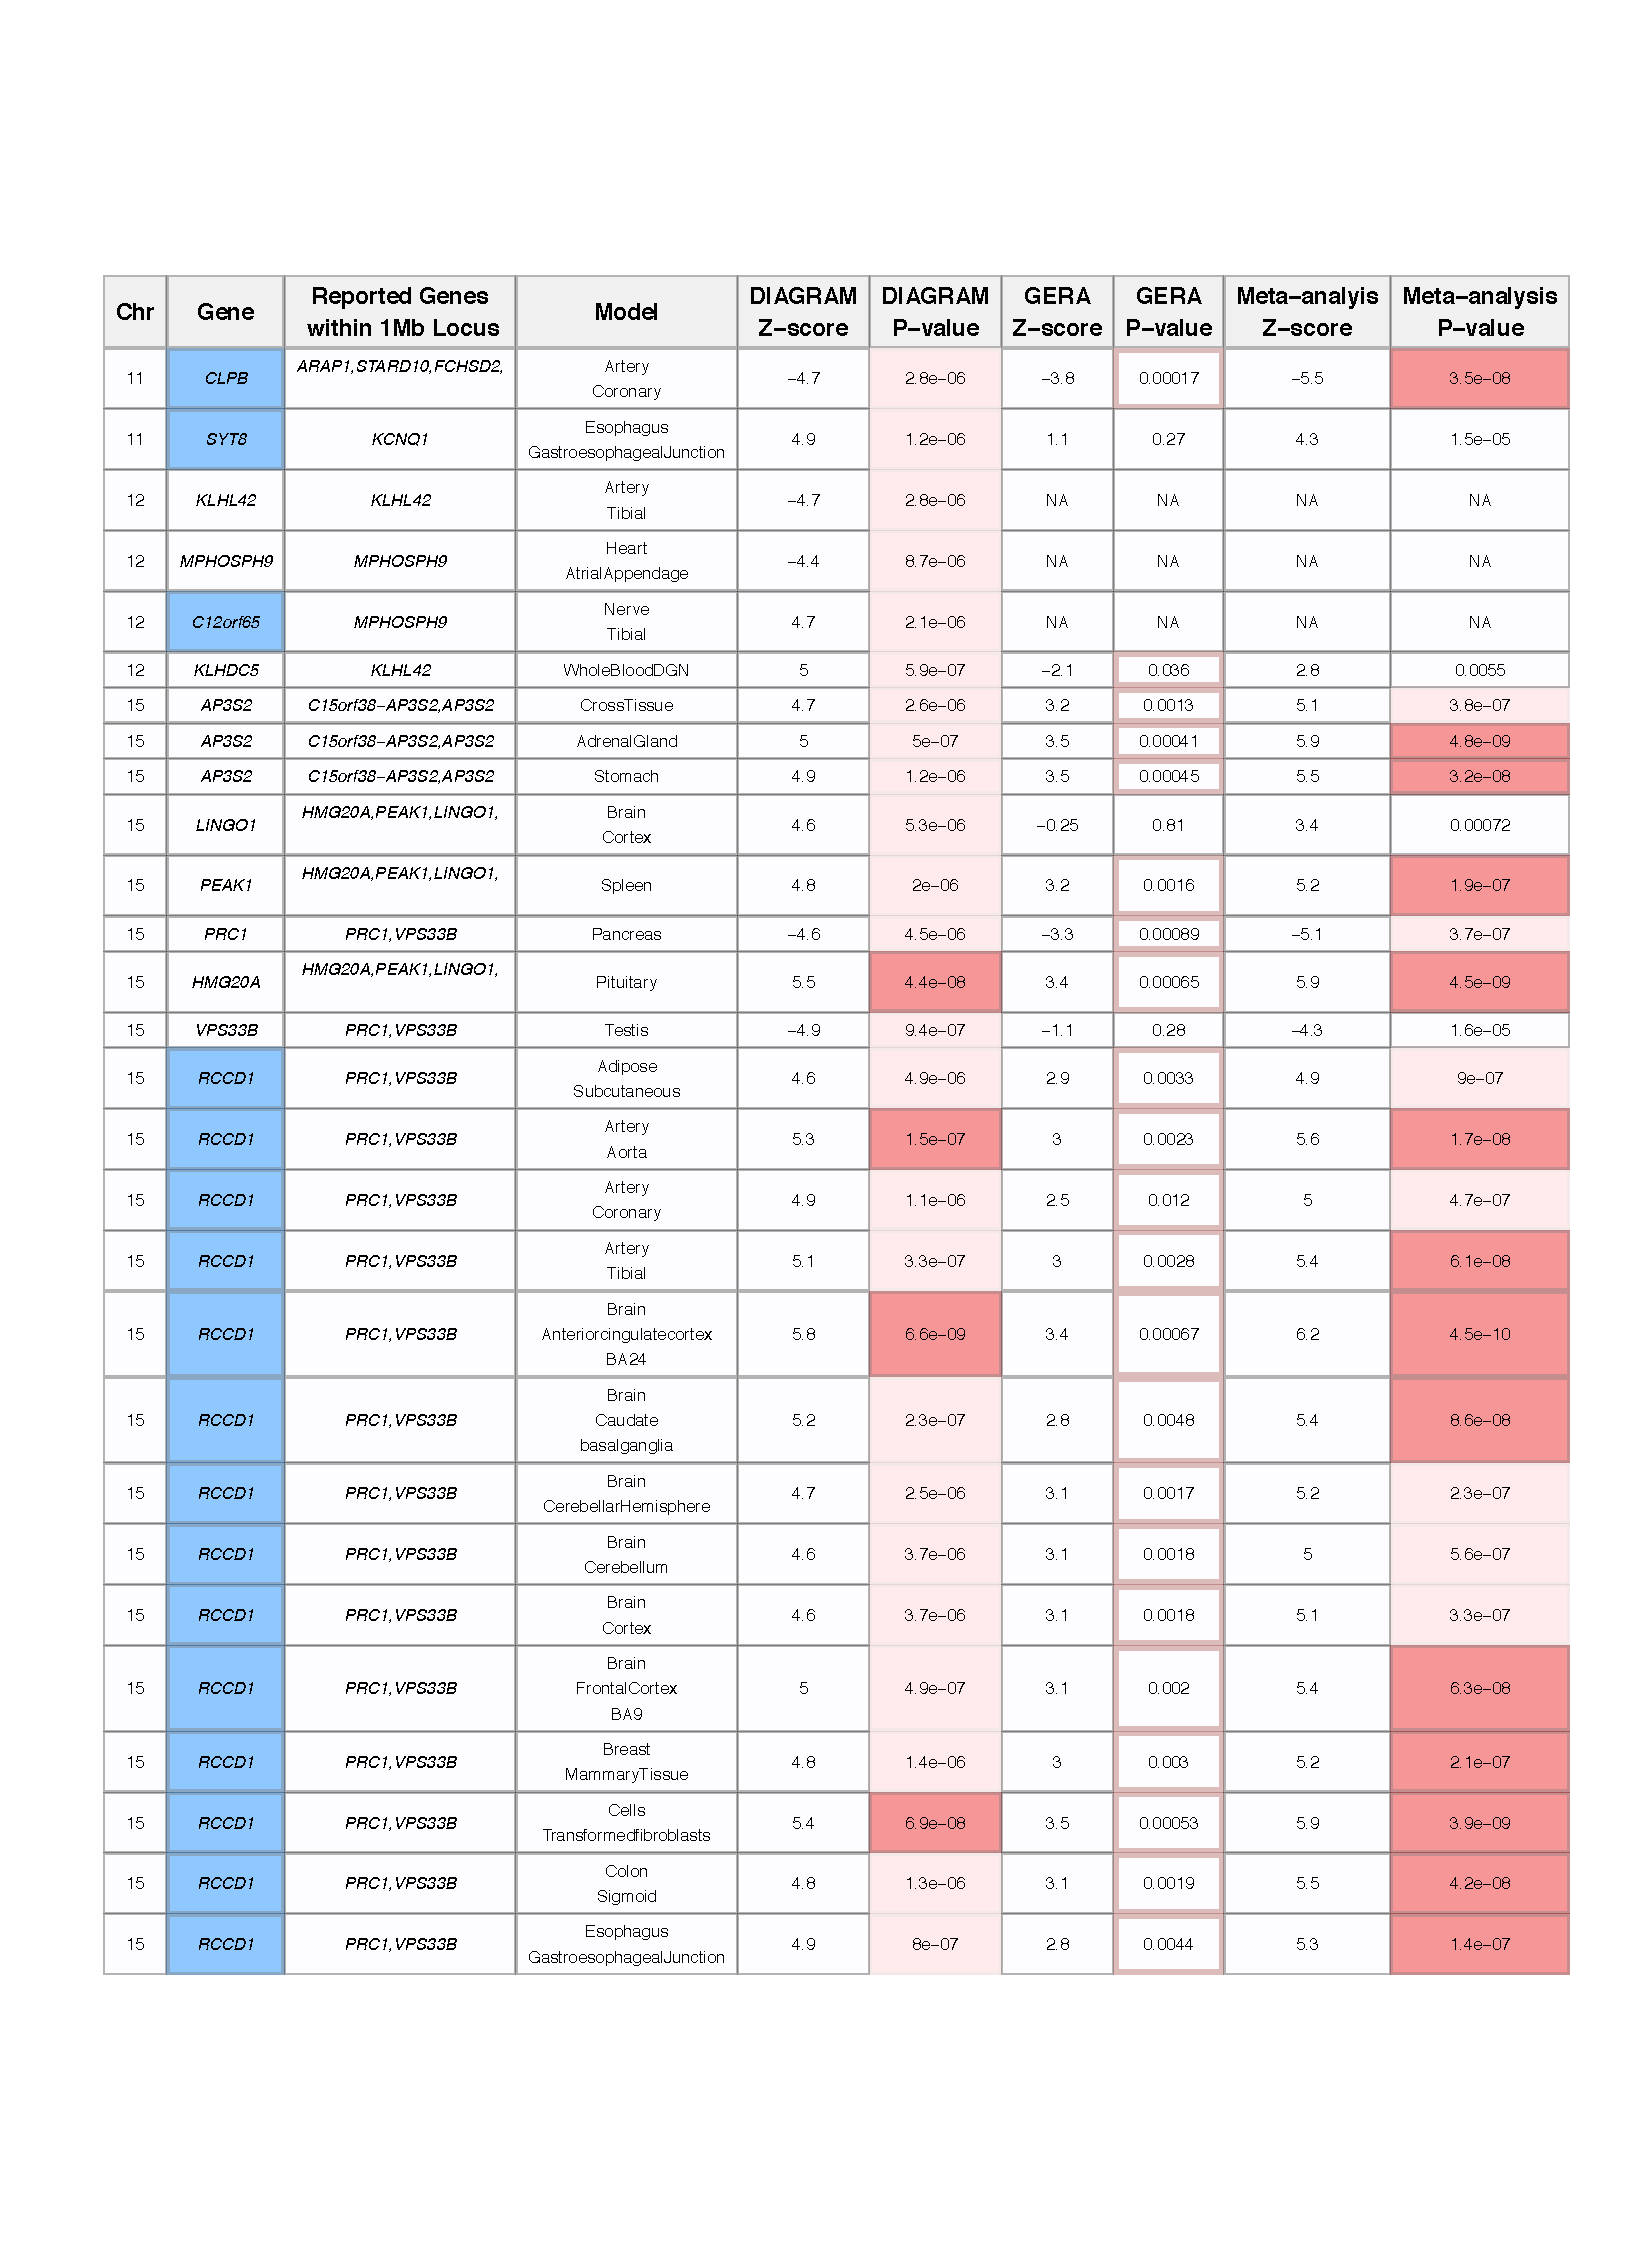
\includegraphics[width=0.95\textwidth]{table1_part3.pdf}
\caption{\textbf{MetaXcan associations with T2D.} Results for genes and corresponding models that meet genome-wide significance \textit{in at least one model} from the DIAGRAM analysis are shown with nearby genes and results from the GERA replication study and meta-analysis of DIAGRAM and GERA Metaxcan associations. Blue shading denotes genes not implicated by the top $1,000$ SNPs from the DIAGRAM trans-ethnic meta-analysis of GWASs. Pink and red shading denote genome-wide significance in one model and across all models, respectively, for the DIAGRAM and meta-analysis. Replication in the GERA study is denoted by a pink outline.} \label{tab:table1.part3}
\end{table}

\begin{table}
\ContinuedFloat
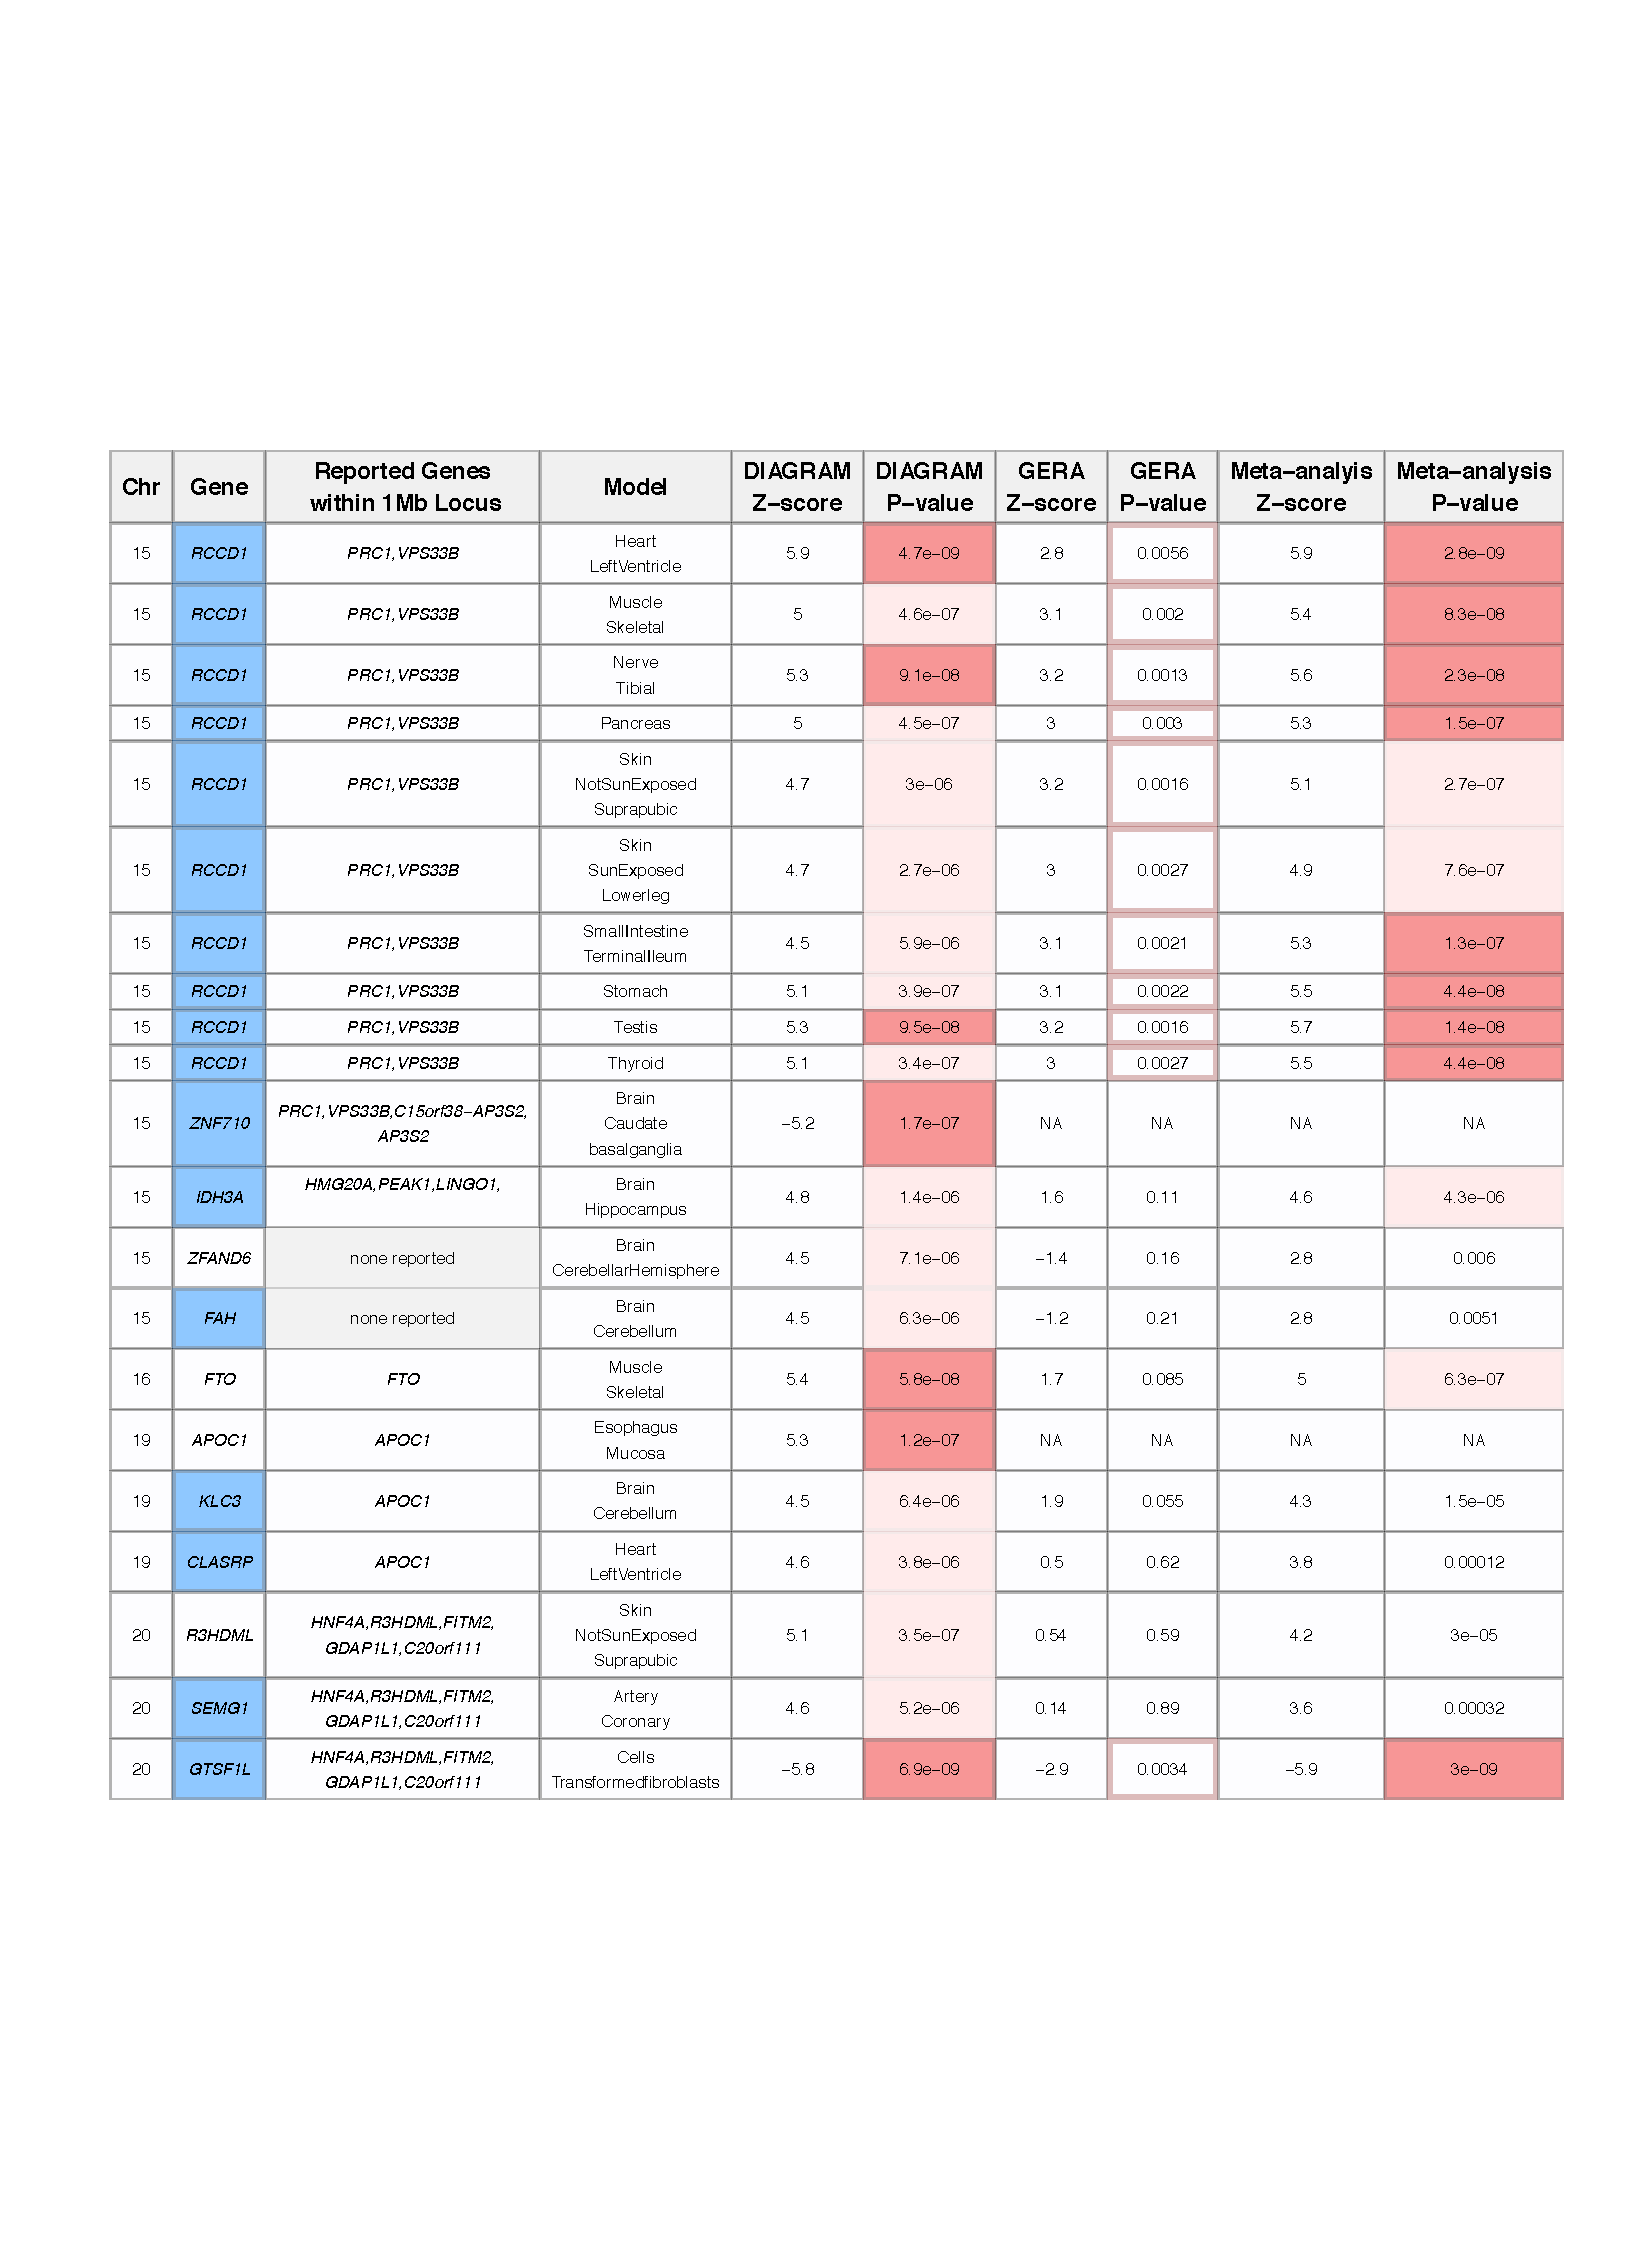
\includegraphics[width=0.95\textwidth]{table1_part4.pdf}
\caption{\textbf{MetaXcan associations with T2D.} Results for genes and corresponding models that meet genome-wide significance \textit{in at least one model} from the DIAGRAM analysis are shown with nearby genes and results from the GERA replication study and meta-analysis of DIAGRAM and GERA Metaxcan associations. Blue shading denotes genes not implicated by the top $1,000$ SNPs from the DIAGRAM trans-ethnic meta-analysis of GWASs. Pink and red shading denote genome-wide significance in one model and across all models, respectively, for the DIAGRAM and meta-analysis. Replication in the GERA study is denoted by a pink outline.} \label{tab:table1.part4}
\end{table}

\end{document}

